%%% Version 3.3 Generated 2016/11/10 %%%
%%% You will need to have the following packages installed: datetime, fmtcount, etoolbox, fcprefix, which are normally inlcuded in WinEdt. %%%
%%% In http://www.ctan.org/ you can find the packages and how to install them, if necessary. %%%
%%%  NB logo1.jpg is required in the path in order to correctly compile front page header %%%

\documentclass[utf8]{frontiersSCNS} % for Science, Engineering and Humanities and Social Sciences articles
%\documentclass[utf8]{frontiersHLTH} % for Health articles
%\documentclass[utf8]{frontiersFPHY} % for Physics and Applied Mathematics and Statistics articles

%\setcitestyle{square} % for Physics and Applied Mathematics and Statistics articles
\usepackage{url,hyperref,lineno,microtype,subcaption,graphicx}
\usepackage[onehalfspacing]{setspace}
\usepackage{color, soul}
\usepackage{amsmath}
\usepackage{booktabs}
\usepackage{multirow}
\usepackage[normalem]{ulem}
\usepackage[toc,page]{appendix}

\DeclareMathOperator*{\argmaxA}{arg\,max}

\linenumbers
\newcommand{\FR}[1]{{\small \textcolor{red}{\hl{FR: #1}}}}

% Leave a blank line between paragraphs instead of using \\


\def\keyFont{\fontsize{8}{11}\helveticabold }
\def\firstAuthorLast{Sample {et~al.}} %use et al only if is more than 1 author
\def\Authors{First Author\,$^{1,*}$, Co-Author\,$^{2}$ and Co-Author\,$^{1,2}$}
% Affiliations should be keyed to the author's name with superscript numbers and be listed as follows: Laboratory, Institute, Department, Organization, City, State abbreviation (USA, Canada, Australia), and Country (without detailed address information such as city zip codes or street names).
% If one of the authors has a change of address, list the new address below the correspondence details using a superscript symbol and use the same symbol to indicate the author in the author list.
\def\Address{$^{1}$Laboratory X, Institute X, Department X, Organization X, City X , State XX (only USA, Canada and Australia), Country X \\
$^{2}$Laboratory X, Institute X, Department X, Organization X, City X , State XX (only USA, Canada and Australia), Country X  }
% The Corresponding Author should be marked with an asterisk
% Provide the exact contact address (this time including street name and city zip code) and email of the corresponding author
\def\corrAuthor{Corresponding Author} 

\def\corrEmail{email@uni.edu}


\begin{document}
\onecolumn
\firstpage{1}

\title[Running Title]{Predicting age with machine learning, using synchronized speech and MEG recordings in children} 

\author[\firstAuthorLast ]{\Authors} %This field will be automatically populated
\address{} %This field will be automatically populated
\correspondance{} %This field will be automatically populated
 
\extraAuth{}% If there are more than 1 corresponding author, comment this line and uncomment the next one.
%\extraAuth{corresponding Author2 \\ Laboratory X2, Institute X2, Department X2, Organization X2, Street X2, City X2 , State XX2 (only USA, Canada and Australia), Zip Code2, X2 Country X2, email2@uni2.edu}

\maketitle

\begin{abstract}

  As language ability develops in children, the cortical structures employed in the brain progressively lateralize into (typically) the left hemisphere. Verb generation tasks have consistently demonstrated this phenomenon in both fMRI and MEG studies using a variety of analysis techniques. With the recent increase in popularity of machine learning and deep neural networks, we consider whether a neural network trained with raw MEG signals can be used to predict the age of children performing a verb-generation task, a monosyllable speech-elicitation task, and a multi-syllabic speech-elicitation task. We further explore what criteria the network uses to make this distinction and compare its performance to a more traditional, feature-based, machine learning pipeline, which is commonly employed in brain-computer-interface applications. We propose two deep networks, one that mimics the feature-based pipeline using convolutional layers, and another that extends this with a recurrent neural network attention mechanism. Our dataset features 92 subjects aged 4-18 recorded using a 151 channel MEG helmet and a single channel of synchronized audio. Our proposed model scores over 97\% binary classification accuracy when distinguishing between greater or less than 10 years of age, and develops spatial filters that consistently emphasize regions localized around the left inferior frontal gyrus.

 \keyFont{ \section{Keywords:} Deep Learning, Machine Learning, Convolutional Neural Networks, MEG, Language Acquisition, Brain Computer Interface, Data Augmentation}
\end{abstract} 

\section{Introduction}

The development of speech from infancy to adulthood is a remarkable and uniquely human process. Language and speech in the adult brain spans a diverse set of regions and interconnections from brain stem to cerebral cortex \cite{GuentherBook, Tourville2011, Hillis}, but higher level language abilities are a typically left-hemisphere lateralized process for approximately 90\% of the general population \footnote{This number can increase to above 95\% in distinctly right-handed individuals, or drop to nearly 70\% in strongly left-handed individuals \cite{GuentherBook}.} \cite{GuentherBook, Kadis2011, Yu2014}. Children develop this lateralization over time and show more bi-lateral activity as an inverse function of age \cite{Kadis2011, Ressel2008}. A common experiment paradigm for demonstrating this development of lateralization is the verb-generation task, which requires a subject to produce a verb they feel conveys meaning related to a stimuli with which they have been provided (e.g. an image) \cite{Kadis2011}. Speech articulation divorced from language is much less lateralized in comparison to {\em higher level} language faculties irregardless of age \cite{GuentherBook}, and in terms of cortical systems, heavily engages the Rolandic cortex to integreate somatosensory and motor control representations to command the speech articulators \cite{GuentherBook}. Despite the fact that this process is less lateralized than higher level language function, non-word monosyllabic, and multisyllabic experiments still show some left-lateralization \cite{Ghosh2008a}. We consider a dataset made up of a combination of a verb-generation task, the monosyllabic utterance /{\em pah}/ and the multisyllable non-word /{\em pah tah kah}/ with overlapping sets of subjects recorded using magnetoencephalography (MEG), in an effort to demonstrate age-related language and speech development. 

Machine learning (ML), especially neural networks has seen a recent surge in popularity as the costs for training has become practical for more scientists \cite{LeCun2015}. ML has been used in brain computer interface (BCI) tasks that typically require a classifier mechanism to make some prediction, and a common merging of language and speech tasks with BCI applications is the prediction of silent speech (imagined or covert) \cite{Sereshkeh2017, Guimaraes2007, Zhao2015a}. A typical pipeline is consistently employed for silent speech with BCIs \cite{RezaeiTabar2016}. First, data are collected and pre-processed using a variety of techniques, such as cropping, trial averaging, normalization, band-pass filtering, and spatial transforms such as principle component analysis (PCA), independent component analysis (ICA) and common spatial patterns (CSP) \cite{Muller-Gerking1999}. The goal of the preprocessing stage is to overcome the low signal-to-noise ratios typical of these types of recordings which complicate training in ML. After these initial steps, features are calculated from these data, of which there are a plethora of successful options, most commonly including spectral characteristics in the canonical brain rhythm bands ($\delta$, $\theta$, $\alpha$, etc.) and statistical moments. Finally, these features and their associated class labels are used to train a classifier. Often, classifiers like support vector machines (SVMs) or logistic regression are used, as they provide convex optimizations that are guaranteed to converge, and are less computationally taxing compared to (large) neural networks. An advantage of this overall approach is that expert knowledge about the data can help circumvent relatively poor signal quality and encourage ML models to distinguish between classes using established signal correlates. However, this comes with potential \emph{bias} of expert knowledge, and the underlying assumptions it may reinforce. In contrast, deep ML models can achieve many of the stages of this pipeline intrinsically. Although these deep-learning architectures are arbitrarily flexible classifiers, when they are trained in an end-to-end fashion, their hierarchical structures can also perform signal-processing in early layers that may be informative when compared to more directed techniques.

Taking an end-to-end machine learning approach to classifying new, perhaps previously difficult, problems that are not just BCI focused may provide new insights into underlying phenomena and also expand the pool of tools available to make sense of the increasingly large data produced by modern non-invasive brain activity recording techniques. Towards this, we propose two new deep neural network architectures trained end-to-end to predict the age of the subjects in our dataset. Since our dataset is of MEG recorded speech tasks, the prediction target of age with this context serves as the method for the ML classifier to find evidence of the development of language itself, rather than age-related distinctions alone.

% ---------------------------------------
\subsection{Related work}

Work specifically investigating end-to-end learning and deep-learning architectures with \emph{EEG} data has become more active recently and our model designs are heavily informed by these works. For instance, convolutional neural networks (CNNs) have shown accuracy improvements in several BCI applications. As a result, a best-practices in architecture seems to be developing along the same lines as our proposed pipeline. Specifically, models that focus on different interconnections between successive layers of temporal convolution and spatial convolution operations in neural networks seem to perform the best in classification. Exclusive spatial filtering in early layers has been used successfully by \cite{Lawhern2017}, \cite{Sun}, and \cite{Schirrmeister2017}. These early spatial filtering layers essentially disentangle the separate sources that are mixed at the cortical surface \cite{ElectricFieldsOfTheBrain_ch5and6}. Schirrmeister {\em et al.} compared three models: a three-layer convolutional network in a configuration that simulates filter-bank common-spatial-filters (FBCSP), a five-layer deep convolutional network using the exponential linear unit (ELU) non-linearity \cite{Clevert} and residual networks (originally described in \cite{He2015a}) \cite{Schirrmeister2017}. Each of these models were trained on the publicly available `BCI competition IV dataset 2a', and the fist two achieved results that surpassed the previous state-of-the-art classification accuracy. These two successful models represent a good example of how a CNN that emulates a feature-based pipeline can successfully be trained from end-to-end. Lawhern {\em et al.} trained multiple CNNs, of equal parameter sizes, to classify four tasks with known characteristic signals, i.e., a P300 visual-evoked potential, error-related negativity, movement-related cortical potentials and sensory motor rhythm \footnote{This is the same dataset used by \cite{Schirrmeister2017} and as a benchmark in our work here.} \cite{Lawhern2017}. They compared the relative rank in performance of each model across all tasks to find the most generally appropriate architecture to train which they dubbed `EEGNet'. Each of their configurations employed a single early layer that performed spatial filtering, and compared models with two subsequent layers with an equal number of parameters, but differences in their span of temporal and spatial dimension. They found layers with receptive fields of $[2 \times 32]$ and $[8 \times 4]$, respectively, where the first dimension corresponded to a spatial dimension span and the second corresponded to a temporal one. Importantly, their optimal configuration employed two extremes of the parameter space they explored. The first kernel had the shortest length receptive field with respect to the spatial dimension, and the second had the shortest length with respect to the temporal dimension. This indicates that a more optimal solution may be found using even more narrowly focused receptive fields (e.g., single dimension convolutions).

Sun {\em et al.} used a CNN to predict the memory performance of their subjects \cite{Sun}. Their subjects were presented a set of spoken nouns, sequentially over headphones, to remember during an initial study session. They were then tested to indicate from 1 to 5 how much they felt they recognized words from a new set that included previously unheard words. They employed a three-layer CNN that, much like the other work above, began with a layer that develops a spatial filter (where their best performance is achieved with a single such filter), and then is followed by an exclusively temporal filter, and finally with a fully connected output layer before a final softmax output layer. They showed that their CNN outperformed a variety of other powerful techniques, including a continuous wavelet transform with an SVM and two fully-connected neural network configurations.

Others have begun to use recurrent neural networks (RNNs) to process and classify BCI tasks recorded with EEG \cite{Bashivan2016}. RNNs are capable of much more complex processing since they are Turing-complete mechanisms, but have not been considered as often as CNNs and more straight-forward feed-forward networks. Bashivan {\em et al.} evaluated a mixed RNN and CNN architecture using EEG recordings of a working memory experiment, where subjects were asked to memorize a set of written characters and then indicate if a single presented character was in the original set \cite{Bashivan2016}. There, the EEG recordings were effectively translated into video streams, where each of the colours red, green, and blue corresponded to azimuthally projected (and then interpolated) images of three frequency bands. A pre-trained image-classifier CNN was used to extract a temporal stream of features and finally a long-short-term memory (LSTM) RNN classified the sequence. Using this approach, the authors claimed to advance the state-of-art for this application from an error rate of $15.3\%$ to $8.9\%$.

Some of these works examine the inner-workings of the models they develop for insights into underlying neural activity that has taken place. The question of what a deep-learning architecture learns is an open and difficult problem, gaining much more research interest in the last few years. Schirrmeister {\em et al.} proposed a method of correlating convolutional filter outputs with activity in frequency bands of interest \cite{Schirrmeister2017}. Their method provides a good start for determining sensitivities to spectral content, but their approach requires strong assumptions as to where the spectral activity is focused. Sun {\em et al.} examine the magnitude of learned weights at incoming layers and find that the largest weights of their model are found over the prefrontal and temporal cortex \cite{Sun}. We consider an alternative approach that has shown some success in visualizing how CNNs identify the class of an image \cite{Yosinski2015}. This approach generates artificial data that maximize the activity of specific neurons through regularized optimization, to understand to what information these neurons are sensitive. %Of particular interest is when this is performed considering the output classes of a network, an ideal example.

\subsection{Objectives}

We present work that proposes and compares deep-learning models, trained end-to-end, against a feature-based approach in identifying the age of children during speech. We focus on a dataset of synchronized MEG and audio recordings during speech elicitation tasks. We also consider different data-augmentation strategies to help enable deep learning models that would otherwise require extremely large datasets, and contrast data that we produce from our most accurate models against real data to gain some insights into the patterns these models develop.

\section{Neural Networks}

Neural networks, in their most general sense, are a computational platform very loosely based on biological neurons. Their smallest functional unit is the {\em neuron}, and these neurons are interconnected in a variety of configurations depending on the application. Each neuron receives a set of incoming numerical values represented as a vector $\boldsymbol{x}$ scaled by some learned set of {\em weights} represented by some vector $\boldsymbol{w}$. Each neuron computes $o = a(\boldsymbol{w}^T\boldsymbol{x}+b)$, where $b$ is a single learned term to bias the weighted inputs and $a$ is some non-linear function (of which many exist, and currently the most common is the rectified linear unit or ReLU \cite{He2015a} due to its computational simplicity). The values of $\boldsymbol{w}$ and $b$ are said to be {\em learned} by using gradient-descent based optimization of a network's output with respect to provided labelled outputs. The calculation of each optimization step of individual weights and biases in a network is determined through the recursive back-propagation algorithm \cite{GoodfellowTextbook}, which propagates error values backwards from the output of a network to each term being optimized. This computational technique has seen a recent explosion in interest (particularly for the purposes of classification tasks) despite their relatively long history \cite{LeCun2015}, and many different unique network configurations exist, but the most important to this work are summarized below.

\subsection{Fully-connected feed-forward neural network}

Feed-forward neural networks (FFNNs) are perhaps the most straight-forward and historically common incarnation of the neural network. This particular configuration consists of layers of parallel (not interconnected) neurons, who feed their outputs to each of the neurons in a subsequent layer. As such, each layer of neurons receive their own set of inputs from the neurons of the previous layer in kind, or if they are the first layer in the sequence, the set of values that make up the input data. 

\subsection{Convolutional neural network}

A convolutional neural network (CNN) \cite{GoodfellowTextbook, LeCun2015} is a variation on the feed-forward neural network that shares incoming weight terms. So rather than a unique weight for each incoming connection to a neuron a smaller set of shared incoming weights are used for all the incoming connections to each neuron in a single layer. Each neuron applies this smaller set of weights to a different subset of the previous layer's neurons. Specifically, the shared set of weights is swept like a convolution operation over the previous layer, and at each step in the convolution is processed by a single neuron of the subsequent layer. This is done to reduce the number of parameters overall, and as a result of the convolution structure, develop translation-invariant features. In contrast, the feed-forward network's operations that are more akin to mask-like operations that are compounded layer over layer into some arbitrary function.

A CNN is said to have layers with a {\em receptive-field} or to have a {\em kernel}, this refers to the number of shared weights (or equivalently, the number of inputs used at each convolution). This kernel takes some {\em stride}, which refers to the number of inputs in the datapoint to proceed ahead before feeding the next subsequent neuron. The number of different kernels (or filters) refers to the number of independent sets of weights learned for each layer (where each filter for the most part has the same receptive field and stride). It is also common to apply pooling layers \cite{Krizhevsky:2012:ICD:2999134.2999257} after convolutional layers to encourage differentiation between filters and translational in-variance of filters, so we apply max-pooling layers after all convolutions used in our architectures unless otherwise noted.

\subsection{Recurrent neural networks and long short term memory cells} \label{sec:rnns}

A recurrent neural network (RNN) is the general term for neural network architectures that posses cyclical connections. The most ubiquitous configuration is one in which a set of neurons (or more commonly, a sub-net of neurons) posses a hidden layer (with respect to the input and output layer of connections) that recurrently connects the output of a neuron (or sub-net) back to itself as an additional input. These networks consist of three layers of connections (weights): an input, an output and a (hidden) recurrent layer. Considering an incoming sequence of $d$-dimensional vectors, the input layer connects each dimension of the vector at step $t$ in the sequence $input_t$, to each of the recurrent neurons (or sub-nets). The output at this point $output_t$ is the concatenated outputs of each recurrent neuron, where each output is a function of $input_t$ and, via their recurrent connections, $output_{t-1}$ for that neuron. In other words, each neuron (or sub-net) in the network receives $d$ incoming input layer connections and a recurrent connection of its previous output. Recursively applying this dependence, $output_t$ is a function on the outputs of the network up to that point $output_0, output_1, ..., output_{t-1}$ and the sequence of inputs that produced each output (and some initial state). RNNs are particularly interesting due to the fact that they are Turing-complete mechanisms. The main disadvantege to RNNs is the difficulty in training. In short, a problem arises where gradient values from the end of the sequence can very easily become too large or too small as it is propagated back through the network and is positively enforced \cite{Hochreiter1997a}. This is known as the exploding/vanishing gradient problem, and although a challenge with nearly any large neural network, it is particularly sinister when training RNNs by using ``Back-Propagation Through Time'' \cite{Hochreiter1997a}. Training RNNs requires the careful design of recurrent sub-nets, that compute the output at each point in the sequence and employ various techniques to minimize this issue.   

The long short-term memory (LSTM) \cite{Hochreiter1997a, GravesRNNBook} recurrent network circumvents the vanishing gradient problem by employing \emph{gating} neurons which preserve values until they are required, and delete values that are determined to be no longer useful. A typical LSTM (and the one we use in the work below) consist of three gate units, the input, forget and output gates. The input gate controls whether new data is to be considered, the forget gate controls whether to preserve or forget a previous value, and the output gate controls whether to feed the internal value of the recurrent unit. These gates are all controlled by some function that is monotonic and continuous from 0 to 1, with 0 indicating a gate that is blocking, and 1 a gate that is not, and accomplish this simply through multiplication. The important point is that each of these gates are differentiable mechanisms, and so can be trained using back-propagation, but using them can preserve values in recurrent units to be modified and used when appropriate in long sequences, without degradation as a result of other incoming data.

\subsubsection{Bi-Directional RNNs}

When RNNs process a sequence, the output at point $t$ is dependent on the previous sequence of inputs $0, 1..., t-1$, but sequences are not always so progressively deterministic. An example would be a sentence, where the meaning of a word is ambiguous earlier in a sentence, but is revealed or clarified by a subsequent word. Bi-directional RNNs essentially employ two stacked LSTM networks, one trained forward through the data and the second trained backwards in time \cite{GravesRNNBook}. The data from both are typically combined through a concatenation of output vectors or summation of outputs (here, we concatenate the outputs).

\subsubsection{Attention} \label{sec:attn_description}

% Definitely want figure for this section

Attention mechanisms have been applied to information retrieval \cite{Moritz}, machine translation \cite{Luong2015}, and speech recognition \cite{Bahdanau}. They are also regularly employed in transduction tasks like image captioning \cite{XuKELVINXU} and visual question answering \cite{Ye2017}. The general principle remains mostly the same across all of these implementations, i.e., to focus a network over a sequence of features by relatively weighting each feature over the entire sequence given the current state of a sequential network (almost always a RNN, but could theoretically be any sequential system). The formulation that tends to be easiest to integrate is a `soft-attention' model \cite{XuKELVINXU}, as it is trained along with the rest of the model using back-propagation. Considering a sequence of features to which we would like to attend, denoted here as $\{f_0, ..., f_{T-1}\}$, and a sequence of current states $\{h_0, ..., h_{T-1}\}$ (in our case the output of an RNN at each step through a sequence of data), \emph{soft-attention} is calculated by first producing an un-normalized {\em energy} vector with length $T$ for each feature $j$ and for each time $t$, as a function of the previous hidden state $h_{t-1}$ and the entire sequence of the feature $j$: 

\begin{equation} \label{eq:attn_nrg}
  e_{t, j} = a(f_{0, j},..., f_{T-1, j}, h_{t-1}),
\end{equation}
Where $a()$ is an arbitrary function\footnote{We use a multi-layer network similar to the original formulation in \cite{XuKELVINXU}, but the number of layers used is a hyperparameter determined during search, and units per layer equal to the number of hidden units with the associated LSTM.}. These vectors are normalized (so that they sum to 1, and range between 0 and 1) using the softmax function. This produces the {\em soft-attention} weights $\alpha_{t,j,t'}$ for each feature $j$ at time $t'$, to produce a new value for the feature $j$ at time $t$:

\begin{equation}
  \alpha_{t,j,t'} =  \frac{\exp(e_{t,j,t'})}{\sum_{i=0}^{T-1}\exp(e_{t,j,i})},
\end{equation}
%Finally the new attention-weighted feature is: 

\begin{equation} \label{eq:attn}
    f_{t,j}' = \sum_{i=0}^{T} f_{i,j} \alpha_{t,j,i}
  \end{equation}
Thus the new input feature $j$ to the RNN at time $t$ is a weighted average of the entire sequence of the feature $j$ determined as a function of the current state and the sequence of $j$ itself.

\section{Data}

\subsection{Primary dataset: Synchronized MEG and speech recordings}

\begin{table}[t]
  \centering
  \begin{tabular}{ l@{}c c c c }
    \toprule
    \textbf{Stimuli} & \textbf{Age range} & \textbf{Subjects} & \textbf{Trials}  & \textbf{M/F Split} \\
    \midrule
    /{\em pah}/~~~                    & $4.1-18.1$   &   $89$   &   $115$   &   $0.45/0.55$ \\
    /{\em pah tah kah}/~~~            & $4.1-18.1$   &   $83$   &   $115$   &   $0.45/0.55$ \\
    VG~~~                             & $5.7-18.0$   &   $28$   &   $81$    &   $0.42/0.58$  \\
    \bottomrule
  \end{tabular}
  \caption{Participant demographics, across stimuli type. The two tasks involve considerable participant overlap.}
  \label{tab:subjects}
\end{table}

These data were originally recorded to examine age- and sex-related developmental language differences in children by \cite{Doesburg2016} and \cite{Yu2014}. Table \ref{tab:subjects} summarizes  participant demographics. Each participant spoke English as their first language and had no known or suspected histories of speech, language, hearing, or developmental disorders, according to their parents. Prior to the experiment, children received two standardized clinical tests: the Peabody Picture Vocabulary Test (PPVT) \cite{Dunn97} and the Expressive Vocabulary Test (EVT) \cite{EVT}. All children's scores were at or above expected scores for their ages on the PPVT and EVT, and their speech showed neither signs of articulatory difficulties nor any significant effect of age, as visualized in Figure \ref{fig:ppvtevt}. In total, 80 participants were right-handed, 5 were left-handed, and 7 were ambidextrous, according to the Edinburgh assessment \cite{Oldfield1971}. %; there is no significant variation of handedness with age.

\begin{figure}[htp]
\includegraphics[width=\columnwidth]{PPVTEVT.pdf}
\caption{Normalized PPVT and EVT scores across ages for all participants ($\mu=100, \sigma=15$). There are neither signs of speech production impairment nor effect of age on these assessments.}
\label{fig:ppvtevt}
\end{figure}

Three distinct speech-elicitation stimuli were used. The first two were of the monosyllable /{\em pah}/ and the multisyllabic sequence /{\em pah tah kah}/, respectively. These were simple enough for young children and are part of the diadochokinetic rate (DDK) test, which can be used to evaluate neuromuscular control in motor speech disorders. Prior to acquisition, the experimenter demonstrated the productions of each stimuli, without word-like prosodic patterns. The third experiment was an overt verb generation (VG) task in English, where subjects were presented with an image with which they were familiar, and were asked to produce a verb associated with the object \cite{Doesburg2016}.

Recordings were made in a sound-proof room, with each participant lying supine in a magnetically shielded room in the Neuromagnetic Lab of the Hospital for Sick Children in Toronto, using a CTF whole-head MEG system (MEG International Services Ltd., Coquitlam, BC, Canada). The system recorded all 151 MEG channels, and a single audio channel, with a sampling rate of 4 kHz.

Doesburg {\em et al.} \cite{Doesburg2016} predicted language ability as an increase in network synchrony, particularly in the theta band with the increase of age during verb-generation (VG) tasks in children and adolescents. They observed a significant increase in the number of synchronous regions with older adolescents, compared with younger children. Yu {\em et al.} \cite{Yu2014} specifically focused on four regions of interest: inferior frontal regions, dorsolateral prefrontal regions, temporal-parietal regions, and superior temporal regions. They noticed distinct profiles of de-synchrony over time in VG tasks for children within five age ranges (i.e., 4-6, 7-9, 10-12, 13-15, and 16-18 years of age).

\subsection{Supplementary dataset: BCI Competition IV, Dataset 2a}

In an effort to compare the potential success of our end-to-end models to previous work, we also trained some of our proposed models using the BCI Competition IV EEG Dataset \cite{Tangermann2012}. This dataset has featured in several other attempts to apply deep learning to neurophysiological data and is freely available online \footnote{http://bnci-horizon-2020.eu/database/data-sets}.

These data consist of EEG recordings of 9 subjects performing 4 different imagined motor tasks: left hand, right hand, both feet, and tongue. These recordings were broken up into two separate sessions for each subject recorded on different days. Each of these sessions consisted of 6 sets of 48 trials separated by a short break, where the 48 trials were 12 executions of each of the 4 tasks. Thus a total of 288 trials were recorded per session. One session is considered training data, and the second is used as evaluation requiring some carry-over performance between days. The recordings consist of 22 EEG electrodes, and 3 monopolar EOG electrodes, all recorded at 250 Hz and bandpass filtered between 0.5 and 100 Hz. Additionally, a 50 Hz notch-filter was used to minimize line noise. The trials themselves are available as 6 second recordings, where the first two seconds consist of presenting each subject a fixation point. At 2s through 3.25s a task stimuli was presented to the subjects. There is additionally some EOG only trials per session that we discard. 

There are several challenges to using this dataset as a benchmark. It uses a different task entirely and contains EEG rather than MEG recordings, so there are far fewer EEG channels than the number of MEG channels from our primary dataset. The participants also come from a different population than the children and adolescents of our primary data. Regardless, we use this dataset to ensure that our model architectures have some sort of generalizability within this domain that can be compared against previous work. 

\section{Methods}

\subsection{Proposed neural network architectures}

\subsubsection{Spatial summary CNN (SCNN)} \label{sec:scnn}

We propose a CNN architecture where spatial convolutions and temporal convolutions are performed separately. This results in a set of spatial filtering components that can be examined independently from temporal features. This also mimics the common feature approach pipeline of: spatial (channel) mixing, applying filter banks to mixed components to develop a set of features and then finally employing some classifier to use these features. In this architecture, the spatial convolutions ultimately span the length of the incoming channels, but rather than being a single linear layer we introduce non-linearity and multiple convolution layers that work together to construct a more flexible spatial filter, but one that still employs weight sharing at each step. We select a hyperparameter indicating the depth of the spatial filter, and then stack convolutional layers, where each layer reduces the spatial dimension until the final layer completely collapses it to a single dimension. After this, a number of temporal filters (i.e., convolutions over the temporal dimension) are applied to the new spatial mapping (the number is also a selected hyperparameter), and an optional average pooling layer to reduce the number of parameters and effectively low-pass filter these new features. Finally, the resulting features are flattened into a single vector and a FFNN classifier is used as an output stage, with the number of layers determined again through hyperparameter search.

The first few layers of the CNN can be seen as a mapping from $R^{T \times C \times 1}$ to $R^{T \times 1 \times S}$ (the spatial filtering) to $R^{T' \times 1 \times F }$ (the temporal filtering) where $T' \leq T$, $C$ is the number of recording channels, $S$ is the number of spatial transformations, and $F$ is the number of temporal filters. In other words, a set $S$ of non-linear spatial transformations are applied to the $C$ channels, and then a set of $F$ temporal filters are applied to these new sequences.

\begin{figure}[htp]
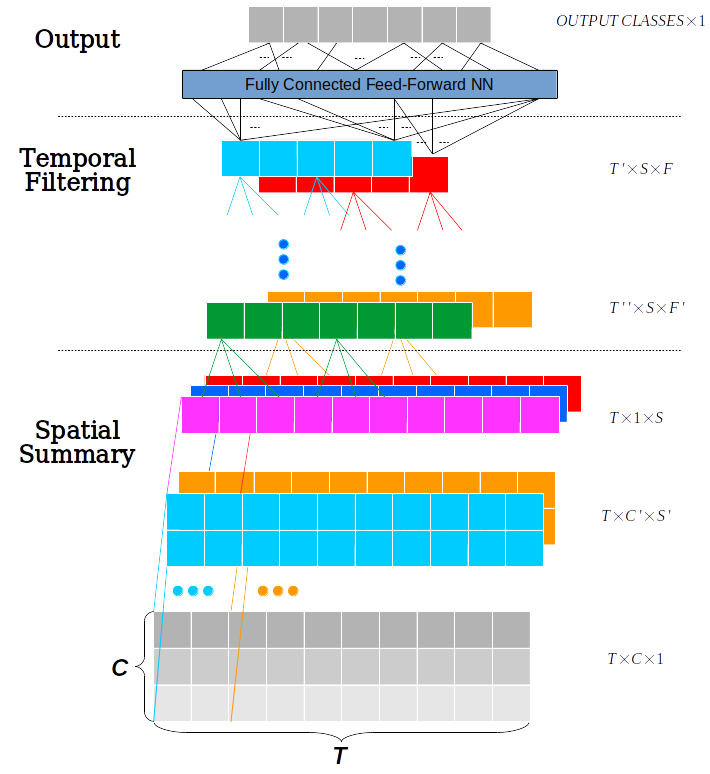
\includegraphics[width=\columnwidth]{SCNN_architecture.png}
\caption{This diagrams shows the Spatial summary convolutional network (which we refer to as SCNN). Processing flows from bottom to top, with the grey array representing a single trial. Each trial has $C$ channels and $T$ (where for our primary dataset: $C=151$ and $T=400$). The architecture is broken down into three stages, a {\em Spatial Summary} stage that performs convolutions exclusively across channels at each timepoint, thus not impacting the number of samples (the second dimension $T$ remains unchanged). Likewise, the {\em Temporal Filtering} stage performs convolutions exclusively across the time dimension. The output stage flattens the resulting output of the previous stages and uses a feed-forward network for final classification.}
\label{fig:scnn_arch}
\end{figure}

Since the actual depth of spatial filtering and temporal filtering operations changes depending on the configuration selected by the hyperparameter search, consider an example architecture with two layers of spatial steps with $K_1, K_2$ kernels for each layer respectively. Let $\boldsymbol{X}$ be our input data with dimensions $T \times C$, where $T$ is the length of our temporal sequence and $C$ is the number of channels recorded. Also, as a result of the two spatial layers, we intend to produce the output $\boldsymbol{X}_{Spatial}$ with dimensions $T \times K_2$ where $K_2$ is the target number of {\em spatial components}. Starting with the first layer, and our $j'^{th}$ kernel $\boldsymbol{w}_{L_1}^j$, which has length $C'$, where $C' < C$, the output of filter $j$ of the first layer at time $t$ is then:

\begin{equation} \label{eq:scnn_s1}
  \boldsymbol{X'}_{t, i, j} = f\left(\sum_{k=0}^{C'} {\boldsymbol{w}_{L_1}^j}_k \boldsymbol{X}_{t,i+k}\right) \footnote{There are no bias terms needed here or later, as batch normalization \cite{Szegedy2015} renders them redundant and is employed throughout.}
\end{equation}

Where $\boldsymbol{X'}$ is a three dimensional tensor of shape $T \times (C-C') \times K_1$ and $f(x)$ is the neuron's non-linear function of choice. There is no integration of any temporal information besides $t$, and that for each kernel there are $C-C'$ sequences of length $T$, of which only the $i'{th}$ is shown above. Next, the second layer consists of kernel vectors $\boldsymbol{w}_{L_2}^s$ of length $C-C'$, which determine component $s$ of $K_2$ at time $t$ as follows:

\begin{equation} \label{eq:scnn_s2}
  {\boldsymbol{X}_{Spatial}}_{t, s} = f(\sum_{i=0}^{C-C'}{\boldsymbol{w}_{L_2}^s}_i \boldsymbol{X'}_{t, i, j})
\end{equation}

The temporal filtering operations behave like eq. \ref{eq:scnn_s1}, but each kernel in the temporal layer is applied across the {\em temporal} dimension of each kernel activation sequence of the previous layer.

\subsubsection{Two-dimensional SCNN}

This architecture extends the SCNN above to data that are represented as 2D interpolated images of shape $D \times D$, rather than single dimensional sequences of channel values. In this architecture, rather than kernels being vectors, they are 2D square tensors that scale patches of the image. As such, \ref{eq:scnn_s1} would instead be expressed:

\begin{equation} \label{eq:s2dcnn_s1}
  \boldsymbol{\hat{X}}_{t, m, n, j} = f(\sum_{m'=0}^{C''} \sum_{n'=0}^{C''} {\boldsymbol{w}_{L_1}^j}_{m', n'} \boldsymbol{X}_{t,m+m',n+n'})
\end{equation}

Which would result in a four-dimensional tensor $\boldsymbol{\hat{X}}$ with dimensions $T \times (C-C'') \times (C-C'') \times K_1$. Similarly modifying \ref{eq:scnn_s1}, the same $X_{Spatial}$ is produced:

\begin{equation} \label{eq:scnn_s2}
  {\boldsymbol{X}_{Spatial}}_{t, s} = f(\sum_{m=0}^{D-C''}\sum_{n=0}^{D-C''}{\boldsymbol{w}_{L_2}^s}_{m,n} \boldsymbol{X'}_{t, m, n, s})
\end{equation}

\subsubsection{Attention LSTM}

We also consider an extension of the SCNN, that uses an LSTM and attention mechanism after the spatial and temporal steps to provide the network a stronger ability to focus on aspects of the signal. In our experiments, we employ an architecture that is very similar to the encoding stage employed in Zhu {\em et al.} for the purpose of image-directed question answering \cite{Zhu}. Those authors used a pre-trained CNN and an LSTM-based encoder that was fed attention weighted inputs. Their attention mechanism provides an average weighting of the different convolutional feature maps which are combined with one-hot encoded word vectors representing the words in the questions.

In contrast, our implementation does not use a pre-trained CNN, but trains convolutional layers at the same time as the rest of the model. The attention serves as a mechanism to closely consider parts of the sequence depending on the state of the LSTM. So the intent is that the LSTM develops some sort of sequential processing that does not need to progress temporally sample by sample, but is flexible to consider any combination of samples that may become appropriate. Functionally, the attention mechanism pre-processes the output of the spatial summary (described in \ref{sec:scnn}) and optionally (a hyperparameter) filtering over time. The pre-processing is an average weighting of the entire temporal sequence of each incoming feature, depending on a function of the current LSTM hidden state and the feature sequence itself. So the input to the LSTM of feature $i$ at some point in the sequence $t$ of $T'$ is:

\begin{equation}
  x_{t,i}^{In} = \sum_{t=0}^{T'} \alpha_{t,i} X_{t,i}^{SCNN}
\end{equation}

Where $\alpha$ is defined in \ref{eq:attn_nrg}. We select whether to use the full LSTM output sequence, or exclusively the last state output as part of our hyperparameter search, and optionally have several fully connected layers before the prediction layer.

\begin{figure}[htp]
  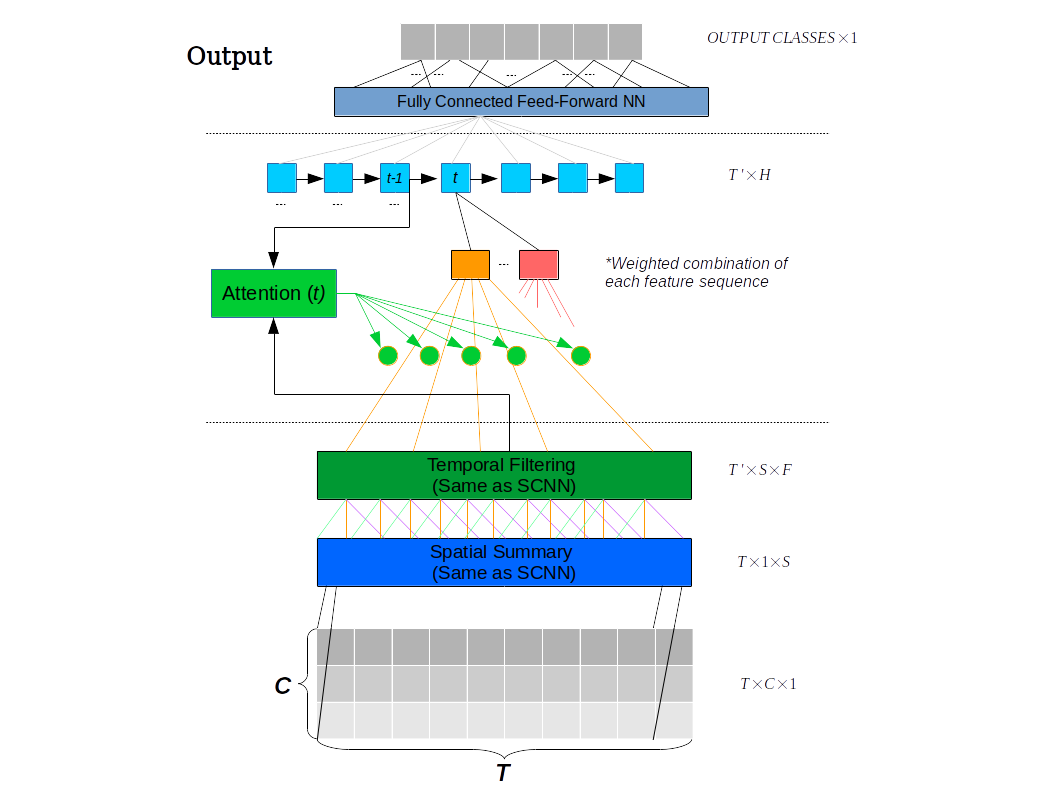
\includegraphics[width=\columnwidth]{ALSTM_architecture.png}
  \caption{This diagrams shows the attention LSTM network. Processing flows from bottom to top, with the grey array representing a single trial. Each trial has $C$ channels and $T$ (where for our primary dataset: $C=151$ and $T=400$). This architecture extends the SCNN presented in \ref{fig:scnn_arch}, where the output of the {\em Temporal Filtering} stage in \ref{fig:scnn_arch} is fed as input to an LSTM enhanced with attention weighted input layer. Finally the output of the LSTM uses a feed-forward network for final classification.}
  \label{fig:alstm_arch}
\end{figure}

\subsection{Data processing}

We resample MEG signals at 200 Hz, and band-pass filter between 0.5 Hz and 100 Hz, to remove offsets and accommodate the canonical ranges of $\delta$, $\theta$, $\alpha$, $\beta$, and $\gamma$ activity. Electrooculography (EOG) artifacts are removed using second order blind identification (SOBI) automated blind source separation as provided by EEGlab \cite{Delorme04eeglab}. This preprocessing step is common to both our feature-based and end-to-end approaches.

To further preprocess our data, for our feature-based approach, we apply info-max independent component analysis (ICA) \cite{Bell1995} to determine statistically independent sub-components of the MEG recordings, across all subjects. This is done by appending MEG recordings for all subjects into a single 151-channel matrix for each of the 3 speech-elicitations: /{\em pah}/, /{\em pah tah kah}/, and the VG task. We then apply the resulting sphering and weight matrices, determined by ICA for each test condition, to each subject's respective recordings. These recordings (i.e., both MEG and audio separately) are then separated into windowed epochs corresponding to frames $-500$ ms to $+1500$ ms around the onset of the stimuli prompt.

\subsection{Feature extraction}

We extract 156 acoustic features and 4681 MEG features from each epoch using openSMILE \cite{Eyben13-RDI}. These are calculated using 50 ms rectangular windows, with a 25 ms overlap resulting in 79 windows per datapoint, they are outlined below.

\subsubsection{Audio features} \label{ssec:audio_features}

Features to represent spectral activity are calculated, for each window, using both a 128-point fast Fourier transform and linear predictive coding coefficients. Additionally, the statistical moments: mean (also absolute mean, quadratic mean, and aforementioned means calculated using only non-zero values), variance, skewness, and kurtosis are calculated. Finally, the root-mean-squared and log of the signal energy are also calculated for each window.

\subsubsection{MEG features}

We extract 31 features for each of the 151 independent components derived from the MEG data. These consist of an 8-point fast Fourier transform, statistical moments, and energy calculation as those used for the audio features \ref{ssec:audio_features}, and the autocorrelation function (ACF) calculated using the fast Fourier transform (FFT) and its inverse (iFFT) for window $w$:

% Probably could use some more discussion of the features here?

\begin{equation}
  ACF(w) = iFFT(|FFT(w)|^2)
  \label{eq1}
\end{equation}

\subsection{Sensor projection}\label{sec:sens_proj}

To better represent the spatial structure of the recordings, we use a series of image representations of the data. The data are originally represented as 2-dimensional arrays whose first dimension corresponds to samples in time, and the second dimension is of length 151, corresponding to the MEG channels in no spatially significant ordering. To represent the spatial nature of the data, the locations of the 151 channels of the MEG sensor array for each experiment are projected using an azimuthal projection (also known as polar projection) onto a two-dimensional grid sized $h \times v$. This transform preserves the distance between each point and a central reference point. The raw values of each sensor are then interpolated over the 2-dimensional image, where each pixel in the image is assigned the value of the nearest (projected) sensor. This generates a series of images, i.e. a three-dimensional datapoint with dimensions $samples \times  h \times v$ where $h$ and $v$ are hyperparameters that we search for before final training. A similar approach was used in Bashivan {\em et al.}, where EEG data were projected and then interpolated into a series of images but, instead of using raw data as we do here, they created multiple channels which represented different spectral features (in their case, the $\theta$, $\alpha$, and $\beta$ frequency bands) \cite{Bashivan2016}. We choose not to take this approach, as this would increase the dimensionality of the problem immensely and, as implemented by Bashivan {\em et al.} \cite{Bashivan2016}, the approach requires a strong assumption of how distinguishing data distributes across particular spectral bands and we intend for the network to distinguish such characteristics without prior knowledge.

\subsection{Data augmentation}

To facilitate end-to-end learning, we employ two techniques that produce multiple usable training points from the same recordings as described below. 

\subsubsection{Cropping}

Here, the entire trial is split into multiple training examples by taking subsections of each trial that still include the event onset. Effectively, rather than one training datapoint for each trial, a sliding window smaller than the length of the trial is used to crop many points, where each point has the event onset localized in a different place. The premise behind this augmentation is that with the event localized in different places, an architecture like a convolutional or recurrent network can learn temporal filters that are agnostic of a specific onset time and thus should be more generalizable. Previous work that has taken a similar approach include Schirrmeister {\em et al.} \cite{Schirrmeister2017} and Sun {\em et al.} \cite{Sun}, but alternatively to our work, they assume a convolutional input stage and provide variable temporal length training points rather than fixed length crops. %We uniformly select a single crop position for each trial every epoch, rather than inflating the number of points in the dataset.

%% \subsubsection{Subsampling}

%% We take advantage of the high sampling rate of the recordings ($4kHz$) being used with respect to the frequency ranges that that we keep  for analysis and examine whether different sub-sampling of the data is a viable augmentation strategy. Filtering is still applied as before to minimize aliasing artifacts, and then we augment the number of samples by re-sampling at a frequency of $200 Hz$

\subsubsection{Noisy sensors}

To our knowledge, there are few examples of data augmentation with respect to the location of channels for training neural networks. Krell \& Kim, developed a rotational strategy of EEG data augmentation where they saw success in increasing classification accuracy for their particular processing chain using rotations in three-dimensional space of $\pm 18^{\circ}$ around the y- and z-axes \cite{Krell2017}. We consider an alternative augmentation strategy that we hypothesize may be more appropriate for MEG data, where the location of a sensor (after projection \ref{sec:sens_proj}) is subject to Gaussian distributed noise (truncated within a single deviation), with the recorded position being the mean of the distribution and variance being a hyperparameter to be selected. As MEG helmets tend to be slightly large for most people, and this effect is exagerated when considering small children such as in our primary dataset, this noisy sensor augmentation is a simple modeling of this source of error to enable better generalization with this higher dimensional data (sensor projection of course increases the dimensionality of the data significantly).

\subsection{Data Analysis}

First, we identify correlations among extracted features, in order to demonstrate evidence for predictive potential. Next, we train a regularized multilinear regression model to predict a subject's age. Finally, we perform two seperate classification tasks. In the first, the children are divided into seven age classifications: 4-5, 6-7, 8-9, 10-11, 12-13, 14-15, and 16 or older. This task demonstrates if a relatively fine-grained distinction can be made by machine learning techniques as to the development of speech production in children. The second classification task is a binary classification tasks predicting whether the child is less than, or greater than 10 years of age. This maximizes the possible accuracy of each model so that the parameters of those trained end-to-end can be examined for the indications it deems to be relevant in distinguishing between early and late developmental speech production stages. Making the binary split at 10 years old  We consider the classification accuracy of both models and additionally consider a {\em within-one} accuracy for the first, fine-grained, classification task. The within-one metric accounts for the continuous nature of our classes: if a model makes a prediction a single class lower or higher than the true class for a datapoint it is still taken to be correct. This will help distinguish models that appear to capture some sense of a trend across labels that are fundamentally a continuous phenomena.

\subsection{Correlation}

We use standard Pearson correlation between the extracted MEG and audio features, for each experiment set separately. We set significance for $p$-values at $\alpha = 10^{-5}$ after Bonferroni correction and consider correlated features as those with absolute value $\text{abs}(r) > 0.2$. For each experiment, we then examine the independent component that had the highest correlations of its features with respect to audio features, to determine if there were any noticeably consistent brain locations that were being emphasized. Furthermore, we compute correlation of MEG and audio features, with respect to age, over the entire data set, to identify features with a potentially stronger predictive capability for later training steps.

\subsection{Model analysis and visualizations} \label{sec:max_act}

Explaining {\em what} a trained neural network has learned is an on-going area of research, and a particularly important one. For neural-network based models to be significantly useful beyond their successes as classifier tools, understanding what they are doing is crucial. There are currently two directions of work that address this, one in which (optionally modified) selections from datasets are fed into an already trained model and the sensitivity of specific layers or neurons are examined, and a second in which artificial data are developed by maximizing the outputs of a trained model with respect to artificial data (with no reliance on training points in particular) \cite{Yosinski2015}. We take the latter approach to develop artificial inputs that maximally activate key points in our models, which involves performing regularized gradient-ascent of an output $f_o(x)$ within the fully trained model with respect to the input $x$. So that we produce an artificial datapoint $x_{max}$ where:

\begin{equation} \label{eq:max_act}
  x_{max} = \argmaxA_x(f_o(x) - R(x))
\end{equation}

Here we summarize any regularization penalties as $R(x)$. \cite{Yosinski2015} show that crucial to the success of this technique is to ensure good prior distributions on the artificial data, so in this spirit we begin with randomly initialized data that have a spectral density that decreases with $1/f$ and zero mean, thus conforming to general encephalographic recordings. We also use L2 regularization on our data-points which helps prevent unbounded growth during the ascent which in effect prevents some strongly relevant features from eclipsings some features that are important but less impactful on the outputs. The iterative maximized input value is then:

\begin{equation} \label{eq:max_act_update}
  \hat{x}_{max} \leftarrow \eta \left(\hat{x}_{max} + \frac{\partial }{\partial x}(f_o(x) - \theta \cdot {}\sum_ix_i^2) \right)
\end{equation}

Where we heuristically select a step increase of $\eta = 0.2$ and L2 regularization of $\theta = 0.05$. We then iterate up to $10,000$ times, stopping if no progress is made for more than 5 steps. Additionally we normalize the derivative in eq. \ref{eq:max_act_update} for each step by its RMS value to make more stable (less oscillatory) progressions.

We construct maximal inputs for two sets of input-output pairs in the trained (using the primary dataset) end-to-end models. The first is between the model's normal input, and the end of the final-most spatial convolution layers, which we then interpolate across true channel locations for our MEG machine to demonstrate a rough localization of spatial components/mixing. The second input-output pair is between the input to the first temporal convolution (the output of the last spatial) and the final model output (classification stage). This is to generate data that highlight temporal features of the patterns of mixed sensors, which we do by calculating a spectrogram (Hann windows with 50 samples overlap and 64 FFT bins) for each component and output class.

\subsection{Model training procedures} \label{sec:train_proc}

Each model is tested using 5-fold cross-validation against a held-out group of subjects. The test subjects are selected to have a similar distribution of the number of trials in each age range. The remaining subjects are ordered based on the number of trials they performed and their trials are distributed across the 5 folds in this order to create an approximately equal number of trials in each fold. The range in number of training points between folds was 3838 through 4078. We quantitatively evaluated the similarity between the 5 folds and test set using a K-sample Anderson-Darling test, where we found $A^2=-0.271$ with $p=0.61$. In the supplemental dataset, the training versus test datasets are separated in advance for intra-subject training.

We use Keras \footnote{https://keras.io/} with a Tensorflow \footnote{https://www.tensorflow.org/} backend to build all of the following models, and use either stochastic gradient descent or the Adam optimizer\cite{Kingma2015} when performing back-propagation updates. When training the neural networks, we select between three different activation functions: the rectified linear unit (ReLU) \cite{He2015a}, the exponential linear unit (ELU) \cite{Clevert}, and the scaled ELU (SELU) \cite{NIPS2017_6698}. All layers are batch-normalized \cite{Szegedy2015} after activation. We additionally employ L2-norm weight regularization for all trainable weights, excluding those of RNNs. We apply dropout \cite{Srivastava2014} after all fully-connected layers, and both max-pooling and spatial dropout \cite{Tompson2015} to all convolutional layers. These techniques are not necessarily applied to the FBCSP-like model from \cite{Schirrmeister2017}, which is reproduced by examining their source code.

All hyperparameter selection is done using Bayesian parameter optimization with Hyperopt \cite{Bergstra2013} including: learning rate, regularization penalty, dropout rates, number of adjacent activations to pool, number and layers of hidden units, receptive fields, and activation functions for all appropriate models. Hyperparameter searches are performed for 100 iterations. Appendix \ref{apdx:hyperparams} has a more detailed description of search spaces used and the specific values for parameters that were ultimately selected.

\section{Results}

\subsection{MEG vs. audio features}

Only $0.0163$\%, $0.0116$\% and $0.132$\% of the $156 \times 4681$ correlations using the /{\em pah}/, /{\em pah tah kah}/ and verb-generation data respectively are significant and beyond the imposed coefficient threshold. This suggests little redundancy between the MEG and audio features as seen by the models that are trained below. Of these significant correlations, three audio features stand out as more strongly correlated to MEG data. These features correspond to sequential FFT bins that represent the frequency range 340-400 Hz. In terms of strongly correlated MEG features: the autocorrelation measure (eq. \ref{eq1}) is the most intensely correlated MEG feature across and is so across three independent components common to all three experiments.

\begin{figure}[htp]
  \centering
  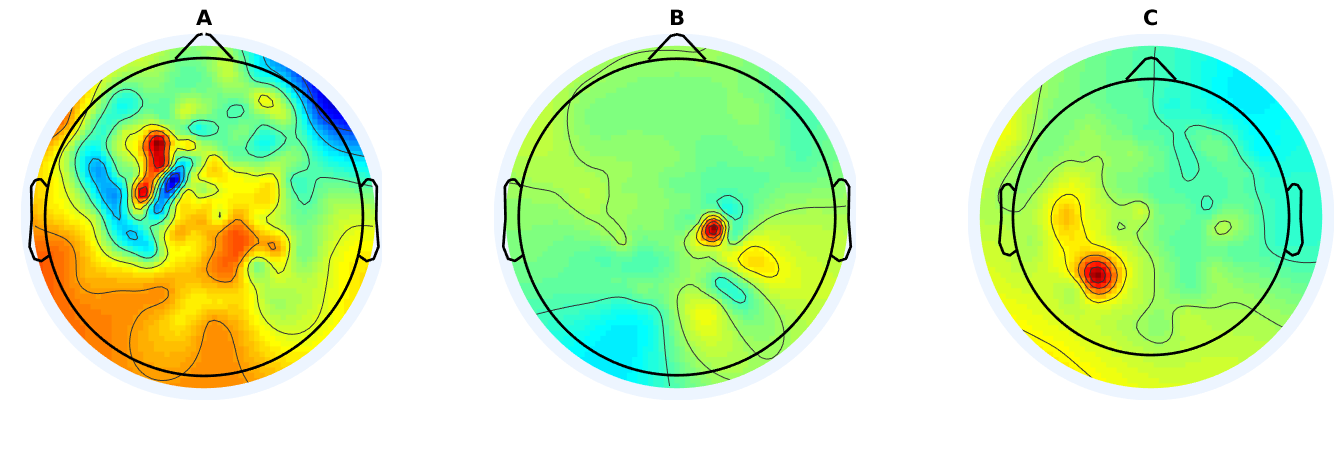
\includegraphics[width=\linewidth]{AllComponents.png}
  \caption{Graphical illustrations (using \cite{Delorme04eeglab}) of the independent components with features most correlated with audio features: A. /{\em pah}/, B. /{\em pah tah kah}/ C. Verb generation experiments. These are generated using the ICA weight matrix interpolated over MEG sensor locations.}
  \label{fig:components}
\end{figure}
 
\subsection{All features vs. age}

When correlating with age, 172 features have significant values, all of which are MEG features. This includes the autocorrelation features of eight ICA components (including the first (highest entropy) component) in addition to the entire available frequency spectrum of four of these components.

The correlation of a single ICA component has correlation coefficients $\text{abs}(r)>0.3$ for nearly all of its features, which is true of no other components considered. Three other ICA components also have features with correlation $\text{abs}(r)>0.3$  for features that corresponded to various mean variants.

\subsection{Age regression}

\begin{table}[htp]
  \centering
   \caption{Root mean squared error (RMSE) and mean absolute error (MAE), in years, of 5-fold cross validation for each of the feature sets. Audio features combined with reduced MEG features show the best prediction capability. Bold indicates the best RMSE.}
  \begin{tabular}{ l | c | c | c | c }
    \toprule
    \textbf{Feature set} & \textbf{RMSE Mean} & \textbf{RMSE Dev.} & \textbf{MAE Mean} & \textbf{MAE Dev.}       \\
    \toprule
        Audio~~~                             & ~~~$4.59$         &     $0.45$     & ~~~$3.34$         &     $0.37$       \\
        MEG~~~                               & ~~~$19.0$         &     $16.5$     & ~~~$9.96$         &     $7.86$       \\
        Audio+MEG~~~                         & ~~~$63.7$         &     $61.0$     & ~~~$63.7$         &     $61.0$       \\

        \midrule
       
        MEG (red.)~~~                        & ~~~$5.51$         &     $2.12$    & ~~~$3.28$          &     $0.30$       \\
        Audio+MEG (red.)~~~                  & ~~~\textbf{2.97}  &     $2.05$    & ~~~\textbf{2.97}         &     $2.05$      \\

    \hline
  \end{tabular}
 % \caption{Root mean squared error (RMSE) and mean absolute error (MAE), in years, of 5-fold cross validation for each of the feature sets. Audio features combined with reduced MEG features show the best prediction capability. Bold indicates the best RMSE.}
  \label{tab:reg_results}
\end{table}

Regressions across the 5 folds suggest that a multilinear regression model trained using both audio and the reduced (i.e., highly correlated) MEG feature sets performs better than either audio or MEG feature sets alone. Without reducing the MEG feature set, regression performance is quite poor. Table \ref{tab:reg_results} shows the means and variances of root mean squared error (RMSE) and mean absolute error (MAE) values on regression, given various combinations of feature sets. There appears to be a marked decrease in error when combining audio features with a reduced set of MEG features. According to a Friedman test considering results for each fold, the difference in MAE is significant with $\chi^2_4=10.72$ and $p<0.03$. Post-hoc pair-wise Nemenyi analysis does not find any significant ($p<0.05$ after single step correction) pair-wise comparisons, but the combined audio and reduced MEG feature set dataset shows $p=0.07$ with respect to the full MEG and combined audio and reduced MEG datasets, indicating some difficulty accepting the null hypothesis in this case. 

\subsection{Age classification}

\subsubsection{Fine-grained prediction}

\begin{table}[htp]
  \caption{Classification accuracy mean and standard deviation across the seven age classes (lower inclusive, higher exclusive): 4-6, 6-8, 8-10, 10-12, 12-14, 14-16, $>$16. Also includes within-one (W1) accuracy mean and standard deviation. Strict accuracy has both feature and end-to-end approaches performing relatively well, but considering the within-one metric the un-augmented and temporal augmentation appear to perform consistently well. Friedman tests of within-one metric rejects the null-hypothesis of all equivalent performances and post-hoc analysis shows the SCNN model trained with the temporally augmented MEG data significantly outperforms the spatially augmented data SCNN and the SCNN trained with Audio data.}
  \makebox[\textwidth]{
  \centering
  \begin{tabular}{l l| c | c | c | c}
    \toprule
    \textbf{Dataset} & \textbf{Model} & \textbf{Mean \%} & \textbf{Dev. \%} & \textbf{W1 Mean \%} & \textbf{W1 Dev. \%}\\
    \toprule
    \multirow{5}{*}{Audio}
                     & Logistic Reg.       & 17.5 & 4.42  & 48.1 & 4.41 \\
                     & Linear SVM          & 17.2 & 5.15  & 54.4 & 1.91 \\
                     & FFNN                & 18.9 & 6.00  & 49.7 & 11.9 \\
                     & LSTM+A              & 23.8 & 7.08  & 58.4 & 6.33 \\
                     & SCNN                & 15.6 & 4.00  & 40.2 & 8.59 \\
    % \midrule
    % \multirow{5}{*}{MEG}
    %                  & Logistic Regression & 16.5 & 6.84 \\
    %                  & Linear SVM          & 19.2 & 6.07 \\
    %                  & Shallow NN          & 27.1 & 0.80 \\
    %                  & LSTM + Attention    & 26.0 & 0.80 \\
    %                  & SCNN                & 24.8 & 8.78 \\

    \midrule
    \multirow{5}{*}{MEG (red.)}
                     & Logistic Reg.        & 27.9 & 2.52  & 49.0 & 9.96 \\
                     & Linear SVM          & 28.5 & 0.79  & 53.0 & 2.82 \\
                     & FFNN                & 28.1 & 5.91  & 51.7 & 8.37 \\
                     & LSTM+A              & 20.7 & 6.90  & 50.1 & 11.6 \\
                     & SCNN                & 22.4 & 4.96  & 53.0 & 3.68 \\
    \midrule
    \multirow{2}{*}{MEG (raw)}
                         & LSTM+A              & 28.1 & 5.00 & 60.0 & 9.11 \\ 
                         & SCNN                & 28.6 & 7.91 & 59.9 & 11.0 \\
    \midrule
    \multirow{2}{*}{MEG (cropping)}
                         & LSTM+A              & 26.3 & 2.07 & 50.2 & 2.36 \\ 
                         & SCNN                & 32.4 & 10.9 & 62.6 & 9.29 \\
    \midrule
    \multirow{1}{*}{MEG (projection)}
                         & SCNN                & 21.9 & 2.20 & 44.0 & 5.10 \\
    \midrule
    \multirow{1}{*}{MEG (proj.+noise)}
                         & SCNN                & 15.0 & 5.10 & 37.4 & 9.83 \\
    \bottomrule
  \end{tabular}}
%  \caption{Classification accuracy mean and standard deviation across the seven age classes (lower inclusive, higher exclusive): 4-6, 6-8, 8-10, 10-12, 12-14, 14-16, $>$16. Also includes within-one (W1) accuracy mean and standard deviation. Strict accuracy has both feature and end-to-end approaches performing relatively well, but considering the within-one metric the un-augmented and temporal augmentation appear to perform consistently well. Friedman tests of within-one metric rejects the null-hypothesis of all equivalent performances and post-hoc analysis shows the SCNN model trained with the temporally augmented MEG data significantly outperforms the spatially augmented data SCNN and the SCNN trained with Audio data.}
  \label{tab:seven_way_results}
\end{table}

The results for models trained across the seven age classes are presented in table \ref{tab:seven_way_results}. Considering the strict accuracy metric alone, there is little differentiation between end-to-end and feature approaches. Both vary in mean scores in the 20-30\% range. The audio dataset, and the spatial projection with augmentation perform somewhat more poorly in this metric than the rest of the datasets and models. The SCNN with cropping augmentation appears to be the most successful model (considering highest mean accuracy), and this holds for the within-one metric as well. However it has quite a large variation and many models score similarly enough for this to mostly be coincidence. Interestingly when considering the within-one metric (W1 in table \ref{tab:seven_way_results}, the models trained with the audio dataset are in fact much more successful and in the case of the SVM perhaps dramatically so when compared to their strict accuracy. This indicates that some sort of pattern is being developed by the model, but is not powerful enough to distinguish among seven classes. The projection and projection+noise augmentation dataset perform quite poorly under both metrics, and additionally required much more training time and had many more parameters, and we would not recommend their use going forward without some change in number of training points or architecture configurations.

Examining the significance of the within-one metric scores using a Friedman test, we can reject that all the scores are equivalent with $\chi^2_{15}=36.494$ $p<0.0015$. Post-hoc Nemenyi analysis shows two significant ($p<0.05$ after single step correction) pairwise comparisons. In both cases the SCNN trained with the cropping augmented raw data significantly outperforms the SCNN trained with the audio dataset and the projection + noise datasets. This adds to an important observation that the models that are intended to be trained with end-to-end data are not {\em aided} by first extracting features, and with the audio dataset and SCNN clearly are {\em disadvantaged} by first extracting features. 

\subsubsection{Binary classification}

\begin{table}[htp]
  \caption{Classification accuracy when constrained to the binary classification problem of $age >= 10$ versus $age < 10$.}
  \centering
  \begin{tabular}{l l | c | c}
    \toprule
    \textbf{Feature set} & \textbf{Model} & \textbf{Mean \%} & \textbf{Dev. \%} \\
    \toprule
    \multirow{5}{*}{Audio}
                         & Logistic Regression    & 54.3 & 6.44  \\
                         & Linear SVM             & 73.9 & 3.45  \\
                         & FFNN                   & 71.7 & 2.44  \\
                         & LSTM + Attention       & 67.5 & 13.9  \\
                         & SCNN                   & 65.9 & 9.35  \\
    \midrule
    \multirow{5}{*}{MEG reduced}
                         & Logistic Regression    & 63.5 & 5.64  \\
                         & Linear SVM             & 69.2 & 5.74  \\
                         & FFNN                   & 66.3 & 4.93  \\
                         & LSTM + Attention       & 72.3 & 1.74  \\
                         & SCNN                   & 69.7 & 7.03  \\
    
    \midrule
    \multirow{2}{*}{Raw Data}
                         & LSTM + Attention    & 92.6 & 5.79  \\ 
                         & SCNN                & 95.1 & 2.31  \\
    \midrule
    \multirow{2}{*}{Temporal Augmentation}
                         & LSTM + Attention    & 93.4 & 0.93  \\ 
                         & SCNN                & 89.2 & 7.93  \\
    
    \bottomrule
  \end{tabular}
%  \caption{Classification accuracy when constrained to the binary classification problem of $age >= 10$ versus $age < 10$.}
  \label{tab:binary_results}
\end{table}

Looking through table \ref{tab:binary_results} we notice what appears to be a very convincing difference in performance between feature-based and end-to-end approaches. The end-to-end approaches all score nearly 90\% or higher accuracy regardless of model used and interestingly, the combination of LSTM + attention model with temporal augmentation appears both highly accurate and consistent. When considering a single fold of the un-augmented raw data and the SCNN model, the accuracy is in fact over 97\%. Analysis with a Friedman test very distinctly shows real performance, with $\chi^2_{13}=52.789$ and $p<10^{-6}$. Despite these promising examinations, post-hoc analysis does not show that the end-to-end models unianimously outperform the feature engineered sets. All end-to-end models do significantly ($p<0.05$ after single-step correction) outperform logistic regression trained with either the audio or reduced MEG feature datasets, and the SCNN trained with raw un-augmented data also significantly outperforms the FFNN trained with the reduced MEG features dataset. Although this is not a unanimous demonstration that the end-to-end models are superior, we see this as a fairly promising indication of performance. Of particular interest are the SCNN models trained without temporal augmentation and the LSTM + attention model with temporal augmentation.

\subsection{Secondary dataset classification}

\begin{table}[t]
  \caption{Classification accuracy of SCNN and LSTM with attention models proposed in this work as compared to the convolutional neural network implementation of a filter bank common spatial pattern (FBCSP) classifier from \cite{Schirrmeister2017}.}
  \centering
  \begin{tabular}{l l | c | c}
    \toprule
    \textbf{Feature set} & \textbf{Model} & \textbf{Mean \%} & \textbf{Dev. \%} \\
    \toprule
    \multirow{3}{*}{No Augmentation}
                         & FBCSP-CNN           & 70.9 & 12.6  \\
                         & SCNN                & 72.6 & 10.7  \\
                         & LSTM + Attention    & 73.3 & 13.6  \\ 
    \midrule
    \multirow{3}{*}{Temporal Augmentation}
                         & FBCSP-CNN           & 65.6 & 12.2  \\
                         & SCNN                & 35.1 & 14.2  \\
                         & LSTM + Attention    & 66.6 & 17.1  \\ 
    \bottomrule
  \end{tabular}
%  \caption{Classification accuracy of SCNN and LSTM with attention models proposed in this work as compared to the convolutional neural network implementation of a filter bank common spatial pattern (FBCSP) classifier from \cite{Schirrmeister2017}.}
  \label{tab:sec_results}
\end{table}

The results in table \ref{tab:sec_results} are meant as a verification that SCNN and LSTM + attention models are more generally applicable to MEG/EEG data and achieve results that are reasonably comparable to state-of-the-art end-to-end machine learning approaches. At first glance there are some increases in classification accuracy, but these are minor with respect to the deviation in performance (which is exceptionally large). Surprisingly, the augmented SCNN model performs extremely poorly with the augmented dataset. Although there appeared to be some drop in its performance against its un-augmented and LSTM + attention counterparts in the binary classification task of the primary dataset, it does not perform remarkably poorly as it does here. In this regard it performs relatively well in the seven-way classification task (and in fact has the highest mean accuracy). After performing paired Wilcoxon signed-rank tests of both SCNN and LSTM + attention models (excluding the dramatic outlier) with respect to the un-augmented CNN as FBCSP implementation, there were no statistically significant comparisons. It appears that these models are at least as good as a comparable state-of-the-art implementation.

\subsection{Model Analysis}

We calculated the maximal activations as described in \ref{sec:max_act} for the model with the highest single fold test accuracy in the binary classification task to minimize creating artificial data that had characteristics that were not pertinent to the task at hand. This resulted in using the SCNN model trained with the second fold of the raw MEG dataset. The full listing of activations is found in Appendix \ref{apdx:max_act} for brevity. Here we focus on components (figure \ref{fig:max_components}) and spectrograms (figures \ref{}) that demonstrate characteristics that are common among the artificial activations.

\begin{figure}[h!]
  \begin{minipage}{0.31\textwidth}
    \centering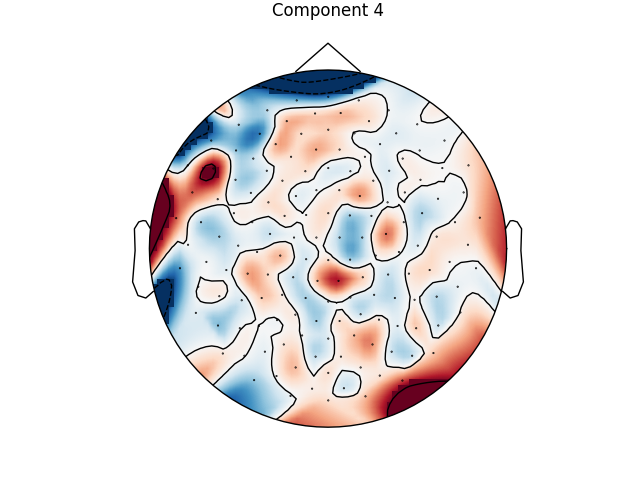
\includegraphics[width=\linewidth]{max_act/4.png}
     \subcaption{}
    %\label{fig:component_4}
  \end{minipage}
  \hspace*{\fill} % separation between the subfigures
  \begin{minipage}{0.31\textwidth}
    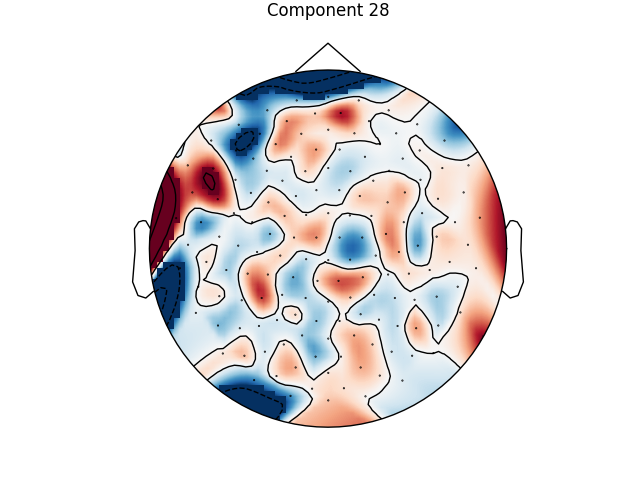
\includegraphics[width=\linewidth]{max_act/28.png}
     \subcaption{}
    %\label{fig:component_28}
  \end{minipage}
   \hspace*{\fill} % separation between the subfigures
   \begin{minipage}{0.31\textwidth}
    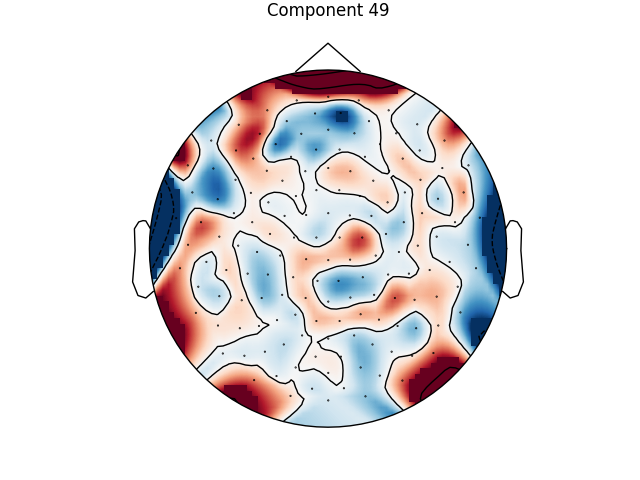
\includegraphics[width=\linewidth]{max_act/49.png}
    \subcaption{}
    %\label{fig:component_49}
  \end{minipage}
  \caption[textfind]{Components (a) and (b) show a common pattern of spatial mixing, with a particularly strong weight localized around channels near the inferior frontal or perhaps dorsolateral prefrontal regions. This region is the only somewhat consistently strongly weighted region that is not exagerated by the edge effects of the interpolation. Component (c) shows a very nearly inverse set of weights compared to (a), in addition to what could be strong weights over the visual cortex (although edge effects of the interpolation make this hard to say). Components were plotted using the MNE python library. \footnotemark} \label{fig:max_components}
\end{figure}
\footnotetext{https://www.martinos.org/mne/stable/index.html}

\begin{figure}
  \begin{minipage}{0.45\textwidth}
    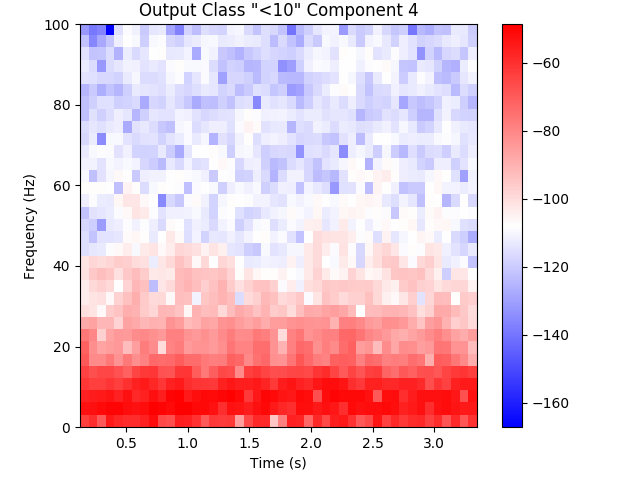
\includegraphics[width=\linewidth]{max_act/artificial_spec_4_0.png}
%    \caption{} \label{fig:art_4_0}
  \end{minipage}
  \hspace*{\fill} 
  \begin{minipage}{0.45\textwidth}
    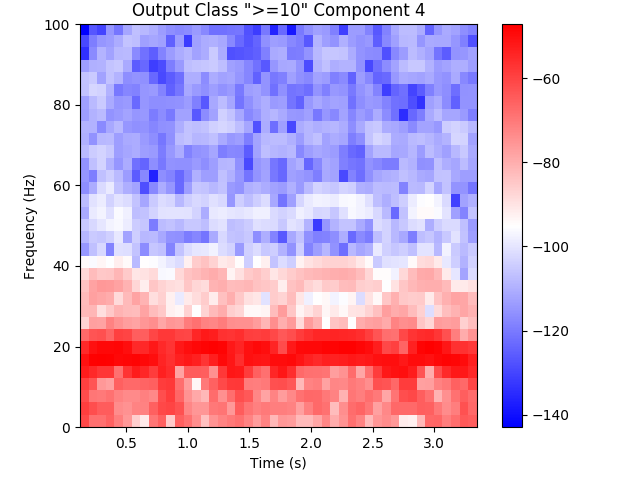
\includegraphics[width=\linewidth]{max_act/artificial_spec_4_1.png}
%    \caption{} \label{fig:art_4_1}
  \end{minipage}
  \vskip\baselineskip
  \begin{minipage}{0.45\textwidth}
    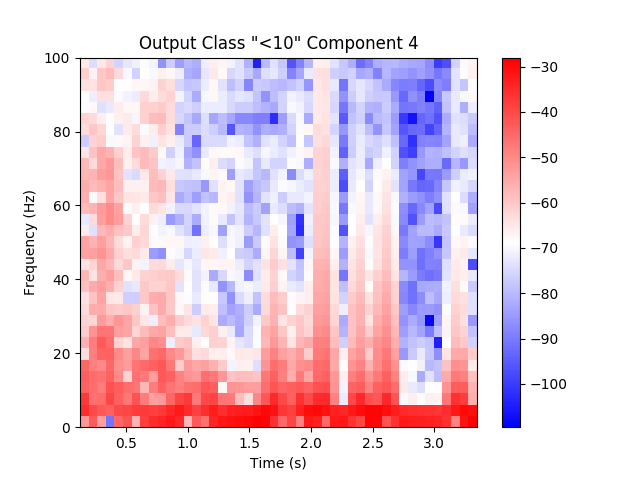
\includegraphics[width=\linewidth]{max_act/real_0_4.png}
%    \caption{} \label{fig:real_4_0}
  \end{minipage}
  \hspace*{\fill} 
  \begin{minipage}{0.45\textwidth}
    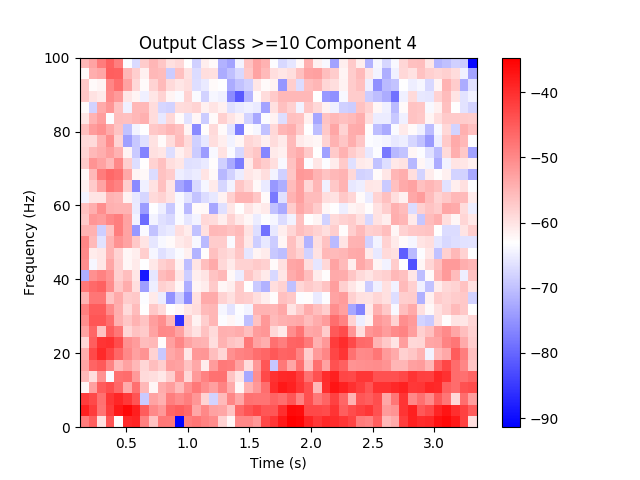
\includegraphics[width=\linewidth]{max_act/real_1_4.png}
%    \caption{} \label{fig:real_4_1}
  \end{minipage}
  \caption{Plots (a) and (b) represent artificially generated data that maximally activate the classes $<10$ and $>=10$ years old respectively with respect to component 4 (plot (a) of figure \ref{fig:max_components}). Plots (c) and (d) show the two real datapoints that most significantly maximized the two classes for the same component.}
  \label{fig:component_4}
\end{figure}

\begin{figure}
  \begin{minipage}{0.45\textwidth}
    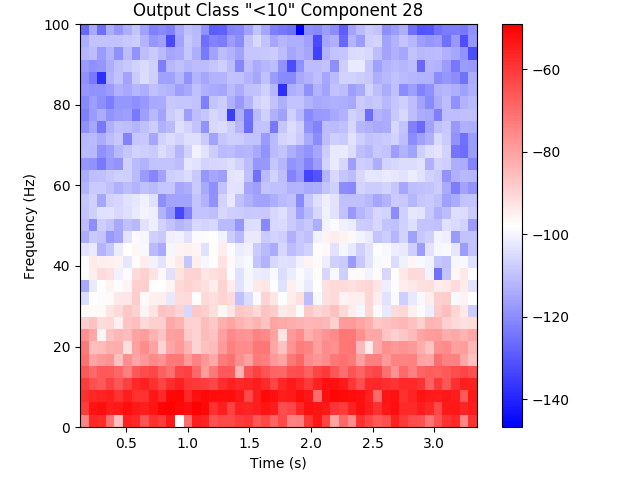
\includegraphics[width=\linewidth]{max_act/artificial_spec_28_0.png}
%    \caption{} \label{fig:art_28_0}
  \end{minipage}
  \hspace*{\fill} 
  \begin{minipage}{0.45\textwidth}
    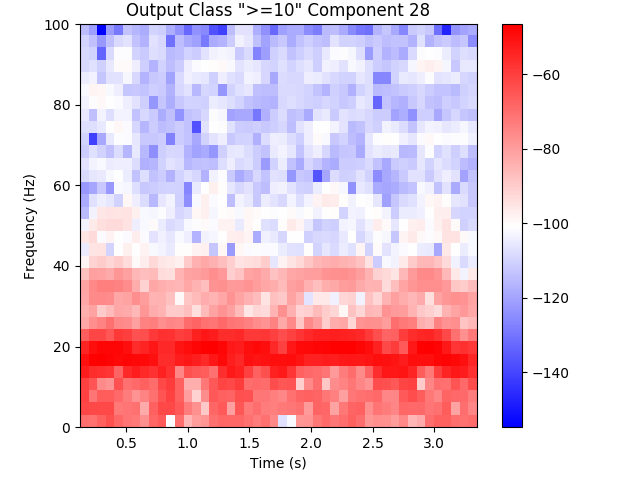
\includegraphics[width=\linewidth]{max_act/artificial_spec_28_1.png}
%    \caption{} \label{fig:art_28_1}
  \end{minipage}
  \vskip\baselineskip
  \begin{minipage}{0.45\textwidth}
    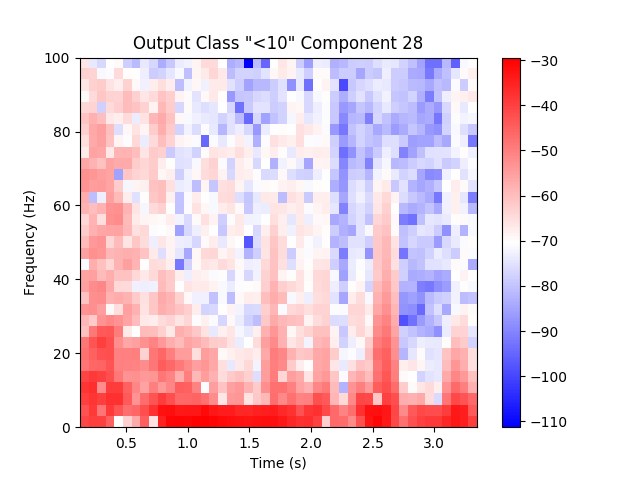
\includegraphics[width=\linewidth]{max_act/real_0_28.png}
%    \caption{} \label{fig:real_28_0}
  \end{minipage}
  \hspace*{\fill} 
  \begin{minipage}{0.45\textwidth}
    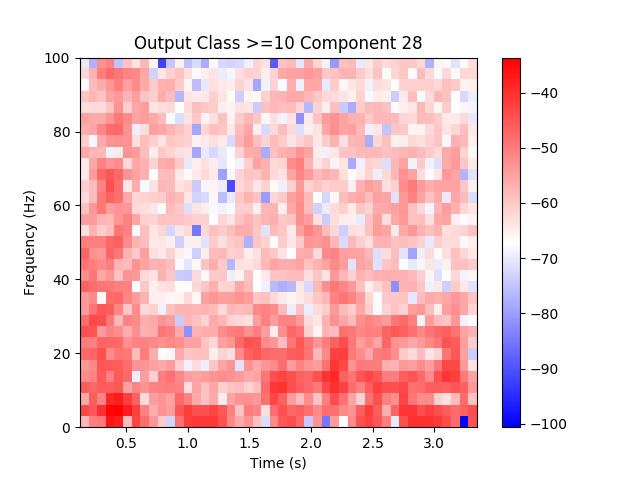
\includegraphics[width=\linewidth]{max_act/real_1_28.png}
%    \caption{} \label{fig:real_28_1}
  \end{minipage}
  \caption{Plots (a) and (b) represent artificially generated data that maximally activate the classes $<10$ and $>=10$ years old respectively with respect to component 28 (plot (b) of figure \ref{fig:max_components}). Plots (c) and (d) show the two real datapoints that most significantly maximized the two classes for the same component.}
  \label{fig:component_28}
\end{figure}

\begin{figure}
  \begin{minipage}{0.45\textwidth}
    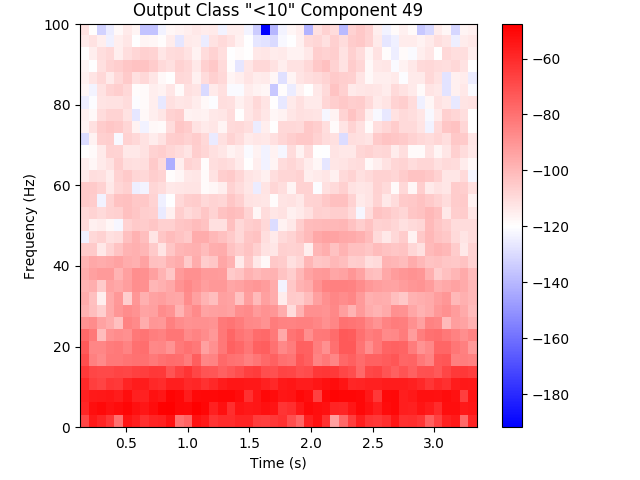
\includegraphics[width=\linewidth]{max_act/artificial_spec_49_0.png}
%    \caption{} \label{fig:art_49_0}
  \end{minipage}
  \hspace*{\fill} 
  \begin{minipage}{0.45\textwidth}
    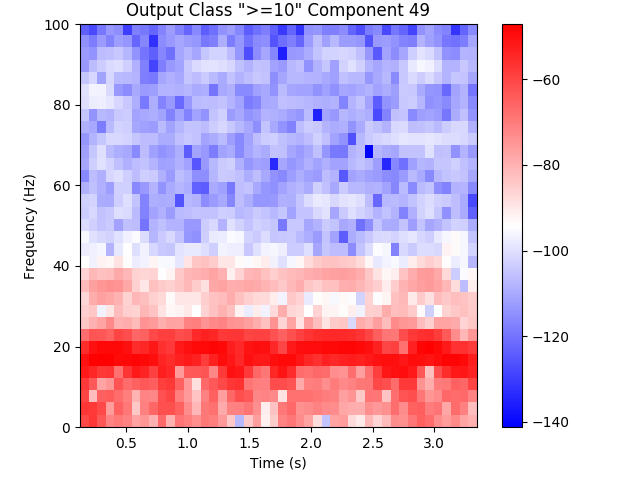
\includegraphics[width=\linewidth]{max_act/artificial_spec_49_1.png}
%    \caption{} \label{fig:art_49_1}
  \end{minipage}
  \vskip\baselineskip
  \begin{minipage}{0.45\textwidth}
    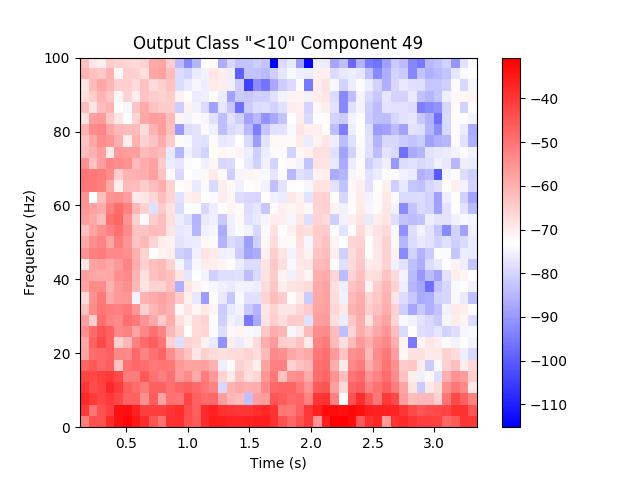
\includegraphics[width=\linewidth]{max_act/real_0_49.png}
%    \caption{} \label{fig:real_49_0}
  \end{minipage}
  \hspace*{\fill} 
  \begin{minipage}{0.45\textwidth}
    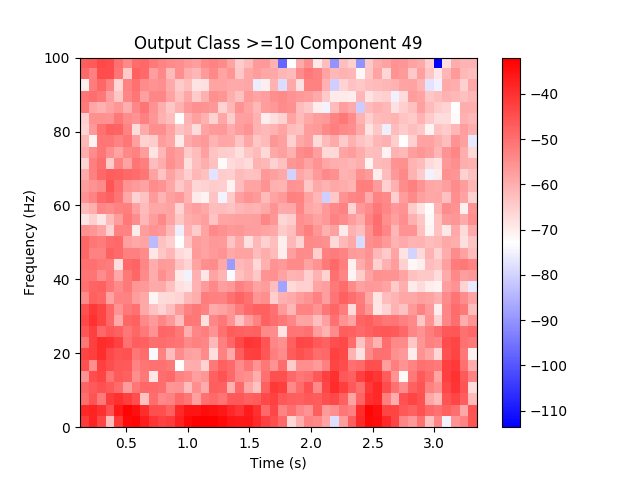
\includegraphics[width=\linewidth]{max_act/real_1_49.png}
%    \caption{} \label{fig:real_49_1}
  \end{minipage}
  \caption{Plots (a) and (b) represent artificially generated data that maximally activate the classes $<10$ and $>=10$ years old respectively with respect to component 49 (plot (c) of figure \ref{fig:max_components}). Plots (c) and (d) show the two real datapoints that most significantly maximized the two classes for the same component.} \label{fig:component_49}
\end{figure}

Throughout the learned components, there is a common patch of strong weights found where what looks like the inferior frontal or perhaps dorsolateral prefrontal regions. All three components shown in figure \ref{fig:max_components} demonstrate this to some degree (although (c) has inverse sign). The artificially generated datapoints show fairly uniform spectrograms across all components, with spectral density concentrated between approximately $0-15$ H$z$ in the $<10$ years old class, and concentration $15-22$ H$z$ for $>=10$ years old. All of the artificial datapoints are very stationary, and show no particular emphasis around the event time $t=1.5s$. The $>=10$ artificial data spectrograms do however show more activity overall in the high $beta$ low $gamma$ rhythms and this is particularly evident in components 4 and 49.

The real data, unlike the artificial data, unsurprisingly is not stationary, and does tend to show a marked change after the $t=1.5s$ mark. Again, much like the artificial data the profiles of each of the components were surprisingly homogeneous.

\section{Discussion}

This work proposes two novel deep neural network architectures that can distinguish between children at different levels of speech development with at least equivalent if not greater accuracy than a feature based-pipeline. These networks also have the advantage of a consolidated training process (they are entirely trained through gradient-descent based optimization without intermediate steps) and also learn parameters that may have direct and interpretable connections to the task they are employed against. They also interestingly perform quite comparably against the state-of-the-art in a completely separate BCI task. 

When establishing the reduced set of MEG features, we evaluated the `optimal' reduced set of features against other subsets of the MEG features to determine if they were justifiably more powerful. First, we randomly extracted a subset of 172 features. Performing multilinear regression on this random selection of features remained insignificantly different than using all features. We also considered a set of the 172 most correlated MEG features among those with $p \geq 10^{-5}$, which accounts for high, but potentially quite variable, correlations. Surprisingly, this improves accuracy slightly on average over using all features, but with a much larger variance. The optimum solution remained to force $p<10^{-5}$ for each correlation. These {\em ad hoc} analyses seem to suggest that increases in performance depend not on merely reducing dimensionality blindly, but on selecting {\em consistently} correlating features.

Performing ICA separately for each stimulus results in different components, naturally. In other words, component $c_i$ with respect to the /{\em pah}/ data is different than component $c_i'$ with respect to the VG data. Future work should consider the sensitivity of any analysis to the stimulus, and be able to generalize ICA analyses that were performed on different data sets, particularly since our approach to end-to-end spatial mixing is done with no consideration for which stimuli were used at training time. Additionally, while we take the spatial patterns from the end-to-end models as similar in principle to ICA, unlike ICA there is no strong source separation premise underlying the neural network approach. In fact neural networks are notorious for developing redundant operations, and at times designers must take many steps to minimize this behaviour.

Although some models succeed in classifying the examples in the primary dataset, many (reasonable) models during hyperparameter searches and initial investigations failed to perform better than random chance. This implies that the architecture selected is of critical importance, and in many cases it will not suffice to try incompatible architectures. We see this as further indication that the application of deep-learning here needs continued development to establish a tool-set of appropriate architectures and stronger guiding principles for this type of data.

During hyperparameter search and initial investigations, we considered {\em label-smoothing} \cite{Pereyra2017} while training the seven-way classification task. This means rather than using {\em one-hot} encoded true labels for the seven classes, we created a discrete pseudo-normal distribution centred at the true label. In practice this meant setting the true label to $0.6$ and its neighbouring classes to $0.2$ (and at the upper and lower ends we set the true label to $0.8$ with its neighbour again $0.2$). This in effect created a distribution that the models were expected to learn, rather than discrete classes. We also considered L2 SVM output layers as described in \cite{Tang2013a}, but found that they performed no better than a softmax output layer and tended if anything to perform slightly worse overall. We also spent some time exploring CNN architectures that developed features using data across time and space, but found very little success with these methods, (these experiments were very preliminary and consisted of a few heuristic selections of parameters). Interestingly the failures were generally not the result of over-fitting, as they found fitting to the training data surprisingly difficult. On the other hand the spatial projection dataset was {\em particularly} susceptible to overfitting to the training data. We believe that the redundant data in this presentation made generalization {\em much} more difficult. Unless considering datasets with many more training points, or employing some more effective regularization techniques we would not recommend proceeding with spatially projected data in future work. 

A somewhat unconventional approach that we took was to train the early convolution layers in conjunction with the subsequent LSTM + attention layers. Previous work favours using pre-trained networks, but this is mostly due to the ubiquity of pre-trained image networks which make the need for re-training an image network unnecessary and time-consuming. We instead have the added challenge of training a subset of the network to calculate a range of spatial and temporal filters, and then learn how to weight the sequence of these features. Future work may benefit from seperating these tasks more to follow previous successes with attention mechanisms. For example the formulation of attention that we borrow from most \cite{Zhu}, is a transduction task that focuses on different aspects of a {\em pre-trained} CNN for image classification and then answers questions about the images using a LSTM+attention layer. This allows them to keep a relatively small training set (one that is less than one million examples) despite such a complex task. An interesting direction for future work might be to develop some general MEG/EEG applicable early layers out of the combination of many different open-access datasets, and then employ LSTMs with attention mechanisms for fine-tuning for a specific task.

Although no statistically significant conclusions can be made as to the power of the SCNN model versus its LSTM + attention counterpart, we should point out that when employing the cropping augmentation, particularly with the secondary dataset, and to a lesser extent the binary classification task, the SCNN performs poorly as compared to the LSTM+attention. This makes some intuitive sense, since the attention mechanism should allow for some insensitivity with respect to event offset, in a more powerful sense than the SCNN, which would rely on a later pooling layer for example to provide this functionality (and thus have a limited range). In practice however, the SCNN trained with cropping augmentation performed much better in the seven-way classification task than any other model.

%Many of the results that are found to be statistically insignificant are not necessarily evidence that some of these models are not strong, and in fact does not imply that they are any worse than other models considered. The fact that there is such a profound increase in overall mean accuracy would typically be taken as an extremely positive result (e.g., the nearly 15\% increase in accuracy between worst case end-to-end binary classification model and the best case feature approach). This highlights the difficulties the machine learning field experiences with statistical significance testing given the relatively minimal number of datapoints provided by cross validation compounded by comparing many models against each other (and this requiring more strict thresholds against type I errors).

As we mentioned in section \ref{sec:max_act}, previous successes with maximal activations such as in Yosinski {\em et al.} employ a heuristic combination of regularization methods that encourage the input data to behave according to patterns the data that will be provided to the network takes \cite{Yosinski2015}. An interesting example Yosinski {\em et al.} provide, is the use of Guassian blur penalization that penalizes the production of images with high spatial frequency \cite{Yosinski2015}. We notice that in fact in our work, the spectrograms we calculate in fact do demonstrate some surprisingly high frequency activity. It may be practical to not just begin with data that have $1/f$ spectral density as we do with our data, but to also penalize deviations from this expectation. There may be more that can be done to regularize artificial data and this warrants further study.

Future work that investigates maximal activations should also take steps to gauge event related synchrony/desynchrony in the context of artificial data, as the current consideration of spectrograms alone is fairly limited. Work in this direction may prove particularly interesting since convolution operations as employed in CNNs are in effect also calculating a correlation measure \cite{GravesRNNBook}.

Towards determining if the /{\em pah}/ and /{\em pah tah kah}/ vocalization trials or the verb generation experiment trials had a greater impact on performance in the end-to-end learning, we trained the raw SCNN model using these datasets separately. Interestingly they seemed to have difficulty outperforming random chance on their own (although these were somewhat earlier model iterations). This suggests that despite being slightly different experiments perhaps at the very least the increase in training data is crucial to enabling the performance of these more powerful ML models.

These results are interesting as a demonstration of the ability of end-to-end models to predict language development, but neural networks show perhaps even greater promise as computational modelling techniques that to some degree mimic the human brain. For example \cite{cichy2016} compare the activations of a image classifier CNN and the MEG and fMRI activity of 15 subjects viewing the same test objects as the CNN. Interesting future work would be to employ new deep neural network architectures that predict speech output or articulator positions with the same data, and explore their connection to real brain structures and/or other speech models such as \cite{Guenther2005}.

\section{Acknowledgements}

We thank Rui Janson for his help performing automated EOG artifacts removal.

\pagebreak

\bibliographystyle{frontiersinSCNS_ENG_HUMS} % for Science, Engineering and Humanities and Social Sciences articles, for Humanities and Social Sciences articles please include page numbers in the in-text citations
%\bibliographystyle{frontiersinHLTH&FPHY} % for Health, Physics and Mathematics articles
\bibliography{frontiers}

\pagebreak

\begin{appendices}
  \chapter{Hyper-parameter search} \label{apdx:hyperparams}

  All hyper-parameter searches were done using hyperopt \cite{Bergstra2013}.
  \section{Search spaces}

\subsection{Logistic Regression}

\begin{table}[h]
  \makebox[\textwidth]{
  \centering
  \label{tab:ss_log}
  \begin{tabular}{ l | c | c | c | c | c }
    \toprule
    \textbf{Parameter} & \textbf{Selection Style} & \textbf{Param. 1} & \textbf{Param. 2} & \textbf{Param. 3} &  \textbf{Resolution} \\
    \toprule
    Batch Size                  &    Uniform    &    $min=1.0$   &  $max=1000$ &  --  & $10$      \\
    Learning Rate               &  Log-Uniform  &   $min=e^{-7}$  &   $max=1$   &  --  & $\infty$  \\
    Momentum                    &  Log-Uniform  &   $min=e^{-7}$  &   $max=1$   &  --  & $\infty$  \\
    Optimizer                   &    Choice \footnotemark     &  SGD \footnotemark  &  Adam  &  --  & --        \\
    L2-Regularization           &  Log-Uniform  &   $min=e^{-4}$  &   $max=1$   &  --  & $\infty$  \\

    \hline
  \end{tabular}}
  \caption{Parameter space for Logistic Regression Models. Although not strictly necessary, these models were trained iteratively in batches like other models.}
\end{table}

\subsection{LinearSVM}

\begin{table}[h]
  \makebox[\textwidth]{
  \centering
  \label{tab:ss_linsvm}
    \begin{tabular}{ l | c | c | c | c | c }
    \toprule
    \textbf{Parameter} & \textbf{Selection Style} & \textbf{Param. 1} & \textbf{Param. 2} & \textbf{Param. 3} &  \textbf{Resolution} \\
    \toprule
    Batch Size                  &    Uniform    &    $min=1.0$   &  $max=1000$ &  --  &  $10$       \\
    Learning Rate               &  Log-Uniform  &   $min=e^{-7}$  &   $max=1$   &  --  &  $\infty$   \\
    Momentum                    &  Log-Uniform  &   $min=e^{-7}$  &   $max=1$   &  --  &  $\infty$   \\
    L2-Regularization           &  Log-Uniform  &   $min=e^{-4}$  &   $max=1$   &  --  &  $\infty$   \\

    \hline
  \end{tabular}}
  \caption{Parameter space for the Linear SVM, trained in batches as with neural network models, all SVMs trained with SGD - Stochastic Gradient Descent with momentum.}
\end{table}

\footnotetext{The ``Choice'' option selects one of the options listed in the parameter columns.}
\footnotetext{Stochastic Gradient Descent \textit{with} momentum.}

\subsection{Feed forward neural network}

\begin{table}[h]
  \makebox[\textwidth]{
  \centering
  \label{tab:ss_ffnn}
    \begin{tabular}{ l | c | c | c | c | c }
    \toprule
    \textbf{Parameter} & \textbf{Selection Style} & \textbf{Param. 1} & \textbf{Param. 2} & \textbf{Param. 3} &  \textbf{Resolution} \\
    \toprule
    Activation                  &    Choice     &    ReLU    & ELU     &  SELU  &  --          \\
    Dropout                     &    Normal     &     0.5    & 0.15    &  --    &  $\infty$    \\
    Batch Size                  &    Uniform    &    $1.0$   & $1000$  &  --    &  $10$        \\
    Optimizer                   &    Choice     &     SGD    & Adam    &  --    &  --          \\
    Learning Rate               &  Log-Uniform  &   $e^{-12}$ & $1$     &  --    &  $\infty$    \\
    Momentum                    &  Log-Uniform  &   $e^{-9}$  & $1$     &  --    &  $\infty$    \\
    L2-Regularization           &  Log-Uniform  &   $e^{-4}$  & $1$     &  --    &  $\infty$    \\

    \hline
  \end{tabular}}
  \caption{Parameter space for the feed forward neural network model.}
\end{table}

\subsection{SCNN}

\begin{table}[h]
  \makebox[\textwidth]{
  \centering
  \label{tab:ss_scnn}
    \begin{tabular}{ l | c | c | c | c | c }
    \toprule
    \textbf{Parameter} & \textbf{Selection Style} & \textbf{Param. 1} & \textbf{Param. 2} & \textbf{Param. 3} &  \textbf{Resolution} \\
    \toprule 
      Activation                  &    Choice     &     ReLU     & ELU               &  SELU  & --          \\
      Dropout                     &    Normal     & $\mu = 0.5$  & $\sigma^2 = 0.15$ &  --    & $\infty$    \\
      Batch Size                  &    Uniform    &   $min=1.0$  & $max=1000$        &  --    &  $10$       \\
      Optimizer                   &    Choice     &     SGD      &        Adam       &  --    & --          \\
      Learning Rate               &  Log-Uniform  & $min=e^{-12}$ & $max=1$           &  --    & $\infty$    \\
      Momentum                    &  Log-Uniform  & $min=e^{-9}$  & $max=1$           &  --    & $\infty$    \\
      L2-Regularization           &  Log-Uniform  & $min=e^{-4}$  & $max=1$           &  --    & $\infty$    \\
      Spatial Units/Layer         &  Log-Uniform  & $min=e^{1.5}$ & $max=e^{5.5}$      &  --    & $2$         \\
      Spatial Layers              &    Uniform    &  $min=1$     & $max=5$           &  --    & $1$         \\
      Temporal Units/Layer        &  Log-Uniform  & $min=e^{1.5}$ & $max=e^{5.5}$      &  --    & $2$         \\
      Temporal Layers             &    Uniform    &  $min=1$     & $max=9$           &  --    & $1$         \\
      Temporal Kernel             &  Log-Uniform  & $min=e^{1}$   & $max=e^{6}$       &  --    & $2$         \\
      Temporal Mean Pool          &    Uniform    & $min=5$      & $max=100$         &  --    & $5$         \\
      Output Layers               &    Uniform    & $min=0$      & $max=3$           &  --    & $1$         \\
      Output Layer 1              &  Log-Uniform  & $min=e^{1.5}$ & $max=e^{5.5}$      &  --    & $2$         \\
      Output Layer 2              &  Log-Uniform  & $min=e^{4}$   & $max=e^{6}$       &  --    & $2$         \\
      Output Layer 3              &  Log-Uniform  & $min=e^{4}$   & $max=e^{6}$       &  --    & $2$         \\
 
     \hline
  \end{tabular}}
  \caption{Parameter space for the SCNN model.}
\end{table}

What appears to be missing in this section is the spatial kernel size. However we select the kernel size as a function of the number of spatial filtering layers. So each layer consists of filters sized ${number of channels}\over{number of layers}$ ($+1$ for output layer as needed to span channel space).

\subsection{LSTM + Attention}

\begin{table}[htp]
  \makebox[\textwidth]{
  \centering
  \label{tab:ss_scnn}
    \begin{tabular}{ l | c | c | c | c | c }
    \toprule
    \textbf{Parameter} & \textbf{Selection Style} & \textbf{Param. 1} & \textbf{Param. 2} & \textbf{Param. 3} &  \textbf{Resolution} \\
    \toprule
      Attention Function Depth    &   Uniform     &      0     & 4       &  --   & $\infty$      \\
      Activation                  &    Choice     &    ReLU    & ELU     &  SELU & --            \\
      Dropout                     &    Normal     &     0.5    & 0.15    &  --   & $\infty$      \\
      Batch Size                  &    Uniform    &    $1.0$   & $1000$  &  --   & $10$          \\
      Optimizer                   &    Choice     &     SGD    & Adam    &  --   & --            \\
      Learning Rate               &  Log-Uniform  &   $e^{-12}$ & $1$     &  --   & $\infty$      \\
      Momentum                    &  Log-Uniform  &   $e^{-9}$  & $1$     &  --   & $\infty$      \\
      L2-Regularization           &  Log-Uniform  &   $e^{-4}$  & $1$     &  --   & $\infty$      \\
      Spatial Units/Layer         &  Log-Uniform  & $min=e^{1.5}$ & $max=e^{5.5}$      &  --    & $2$         \\
      Spatial Layers              &    Uniform    &  $min=1$     & $max=5$           &  --    & $1$         \\
      Temporal Units/Layer        &  Log-Uniform  & $min=e^{1.5}$ & $max=e^{5.5}$      &  --    & $2$         \\
      Temporal Layers             &    Uniform    &  $min=1$     & $max=9$           &  --    & $1$         \\
      Temporal Kernel             &  Log-Uniform  & $min=e^{1}$   & $max=e^{6}$       &  --    & $2$         \\
      Temporal Mean Pool          &    Uniform    & $min=5$      & $max=100$         &  --    & $5$         \\
      Output Layers               &    Uniform    & $min=0$      & $max=3$           &  --    & $1$         \\
      Output Layer 1              &  Log-Uniform  & $min=e^{1.5}$ & $max=e^{5.5}$      &  --    & $2$         \\
      Output Layer 2              &  Log-Uniform  & $min=e^{4}$   & $max=e^{6}$       &  --    & $2$         \\
      Output Layer 3              &  Log-Uniform  & $min=e^{4}$   & $max=e^{6}$       &  --    & $2$         \\
      LSTM Output                 &    Choice     &  Final Step & Entire Sequence & -- & -- \\
      Attention Units/Layer       &  Log-Uniform  & $min=e^{1.5}$ & $max=e^{5.5}$      &  --    & $2$         \\
      Attention Hidden Layers            &    Uniform    & $min=0$      & $max=5$           & -- & $1$             \\
    \hline
  \end{tabular}}
  \caption{Parameter space for the LSTM with attention weighted SCNN features model.}
\end{table}

The LSTM+Attention model must in addition to the parameters of the SCNN model, select whether to use the entire sequence of outputs of the LSTM, or to only use the final output of the sequence. Attention function above referes to the function $a()$ from section \ref{sec:attn_description}.

\subsection{Spatial 2D CNN}

\begin{table}[h]
  \makebox[\textwidth]{
  \centering
  \label{tab:ss_Scnn}
    \begin{tabular}{ l | c | c | c | c | c }
    \toprule
    \textbf{Parameter} & \textbf{Selection Style} & \textbf{Param. 1} & \textbf{Param. 2} & \textbf{Param. 3} &  \textbf{Resolution} \\
    \toprule 
      Activation                  &    Choice     &     ReLU     & ELU               &  SELU  & --          \\
      Dropout                     &    Normal     & $\mu = 0.5$  & $\sigma^2 = 0.15$ &  --    & $\infty$    \\ 
      Batch Size                  &    Uniform    &   $min=1.0$  & $max=1000$        &  --    &  $10$       \\
      Optimizer                   &    Choice     &     SGD      &        Adam       &  --    & --          \\
      Learning Rate               &  Log-Uniform  & $min=e^{-12}$ & $max=1$           &  --    & $\infty$    \\
      Momentum                    &  Log-Uniform  & $min=e^{-9}$  & $max=1$           &  --    & $\infty$    \\
      L2-Regularization           &  Log-Uniform  & $min=e^{-4}$  & $max=1$           &  --    & $\infty$    \\
      Spatial Units/Layer         &  Log-Uniform  & $min=e^{1.5}$ & $max=e^{5.5}$      &  --    & $2$         \\
      Spatial Layers              &    Uniform    &  $min=1$     & $max=5$           &  --    & $1$         \\
      Temporal Units/Layer        &  Log-Uniform  & $min=e^{1.5}$ & $max=e^{5.5}$      &  --    & $2$         \\
      Temporal Layers             &    Uniform    &  $min=1$     & $max=9$           &  --    & $1$         \\
      Temporal Kernel             &  Log-Uniform  & $min=e^{1}$   & $max=e^{6}$       &  --    & $2$         \\
      Temporal Mean Pool          &    Uniform    & $min=5$      & $max=100$         &  --    & $5$         \\
      Output Layers               &    Uniform    & $min=0$      & $max=3$           &  --    & $1$         \\
      Output Layer 1              &  Log-Uniform  & $min=e^{1.5}$ & $max=e^{5.5}$      &  --    & $2$         \\
      Output Layer 2              &  Log-Uniform  & $min=e^{4}$   & $max=e^{6}$       &  --    & $2$         \\
      Output Layer 3              &  Log-Uniform  & $min=e^{4}$   & $max=e^{6}$       &  --    & $2$         \\
      Grid Height/Width           &    Uniform    & $min=10$      & $max=50$           &  --    & $5$         \\
      Sensor Position Var. \footnotemark &    Normal     & $\mu = 0.05$  & $\sigma^2 = 0.01$ &  --    & $\infty$    \\ 
     \hline
  \end{tabular}}
  \caption{Parameter space for the Spatial 2D CNN.}
\end{table}

\footnotetext{Only applies to the noise augmentation model. This parameter determines the covariance (the noise is symmetrical in horizontal and vertical directions) of the sensor locations.}

\section{Best Models}

\subsection{Audio}

\subsubsection{Logistic Regression}

\begin{itemize}
\item Optimizer: Adam
\item Learning Rate: $0.0181$
\item L2 regularization: $0.598$
\item Batch Size: $210$
\end{itemize}

\subsubsection{Linear SVM}

\begin{itemize}
\item Optimizer: Adam
\item Learning Rate: $0.0608$
\item L2 regularization: $0.0213$
\item Batch Size: $910$
\end{itemize}

\subsubsection{Feed Forward Neural Network}

\begin{itemize}
\item Optimizer: Adam
\item Learning Rate: $1.46 \times 10^{-5}$
\item L2 regularization: $9.14 \times 10^{-4}$
\item Batch Size: $40$
\item Activation: SELU
\item Dropout: $0.33$
\end{itemize}

\subsubsection{SCNN}

\begin{itemize}
\item Optimizer: SGD + Momentum
\item Learning Rate: $5.13 \times 10^{-4}$
\item Momentum: $0.0046$
\item L2 regularization: $0.111$
\item Batch Size: $160$
\item Activation: ReLU
\item Dropout: $0.45$
\item Spatial Filters per Layer: $17$
\item Spatial Filtering Layers: $3$
\item Temporal Filters per Layer: $172$
\item Temporal Filtering Layers: $5$
\item Temporal Kernel Size: $2$
\item Temporal Average Pooling Size: $20$
\item Fully Connected Output Layers: $3: [10, 290, 50]$
\end{itemize}

\subsubsection{LSTM + Attention}

\begin{itemize}
\item Optimizer: SGD + Momentum
\item Learning Rate: $2.04 \times 10^{-4}$
\item Momentum: $0.0214$
\item L2 regularization: $0.0216$
\item Batch Size: $140$
\item Activation: ReLU
\item Dropout: $0.48$
\item Spatial Filters per Layer: $108$
\item Spatial Filtering Layers: $2$
\item Temporal Filters per Layer: $230$
\item Temporal Filtering Layers: $9$
\item Temporal Kernel Size: $4$
\item Temporal Mean Pooling Size: $20$
\item Fully Connected Output Layers: $3: [190, 370, 120]$
\item Use only final LSTM step
\item Attention Function Layer Width: $244$
\item Attention Hidden Layers: $2$
\end{itemize}

\subsection{MEG extracted features}

\subsubsection{Logistic Regression}

\begin{itemize}
\item Optimizer: SGD + Momentum
\item Learning Rate: $0.0243$
\item Momentum: $0.0026$
\item L2 regularization: $0.517$
\item Batch Size: $650$
\end{itemize}

\subsubsection{Linear SVM}

\begin{itemize}
\item Optimizer: SGD + Momentum
\item Learning Rate: $0.0667$
\item Momentum: $0.154$
\item L2 regularization: $0.508$
\item Batch Size: $510$
\end{itemize}

\subsubsection{Feed Forward Neural Network}

\begin{itemize}
\item Optimizer: Adam
\item Learning Rate: $0.0016$
\item L2 regularization: $0.0211$
\item Batch Size: $5$
\item Activation: ELU
\item Dropout: $0.59$
\end{itemize}

\subsubsection{SCNN}

\begin{itemize}
\item Optimizer: SGD + Momentum
\item Learning Rate: $0.0094$
\item Momentum: $0.00298$
\item L2 regularization: $0.0477$
\item Batch Size: $40$
\item Activation: ELU
\item Dropout: $0.59$
\item Spatial Filters per Layer: $10$
\item Spatial Filtering Layers: $2$
\item Temporal Filters per Layer: $24$
\item Temporal Filtering Layers: $1$
\item Temporal Kernel Size: $12$
\item Temporal Average Pooling Size: $55$
\item Fully Connected Output Layers: $0$
\end{itemize}

\subsubsection{LSTM + Attention}

\begin{itemize}
\item Optimizer: SGD + Momentum
\item Learning Rate: $7.45 \times 10^{-5}$
\item Momentum: $0.00213$
\item L2 regularization: $0.0216$
\item Batch Size: $20$
\item Activation: ReLU
\item Dropout: $0.56$
\item Spatial Filters per Layer: $7$
\item Spatial Filtering Layers: $2$
\item Temporal Filters per Layer: $4$
\item Temporal Filtering Layers: $9$
\item Temporal Kernel Size: $4$
\item Temporal Mean Pooling Size: $20$
\item Fully Connected Output Layers: $2: [38, 130]$
\item Use only final LSTM step
\item Attention Function Layer Width: $18$
\item Attention Hidden Layers: $1$
\end{itemize}

\subsection{Raw MEG}

\subsubsection{SCNN}

\begin{itemize}
\item Optimizer: Adam
\item Learning Rate: $0.00048$
\item L2 regularization: $0.0041$
\item Batch Size: $40$
\item Activation: SELU
\item Dropout: $0.74$
\item Spatial Filters per Layer: $60$
\item Spatial Filtering Layers: $2$
\item Temporal Filters per Layer: $10$
\item Temporal Filtering Layers: $6$
\item Temporal Kernel Size: $22$
\item Temporal Average Pooling Size: $10$
\item Fully Connected Output Layers: $3: [6, 170, 70]$
\end{itemize}

\subsubsection{LSTM + Attention}

\begin{itemize}
\item Optimizer: SGD + Momentum
\item Learning Rate: $6.72 \times 10^{-5}$
\item Momentum: $0.97$
\item L2 regularization: $0.0061$
\item Batch Size: $20$
\item Activation: ReLU
\item Dropout: $0.55$
\item Spatial Filters per Layer: $76$
\item Spatial Filtering Layers: $3$
\item Temporal Filters per Layer: $136$
\item Temporal Filtering Layers: $8$
\item Temporal Kernel Size: $46$
\item Temporal Mean Pooling Size: $14$
\item Fully Connected Output Layers: $3: [32, 180, 230]$
\item Use entire LSTM sequence.
\item Attention Hiden Layers: $0$
\end{itemize}

\subsection{MEG Temporal Augmentation}

\subsubsection{SCNN}

\begin{itemize}
\item Optimizer: Adam
\item Learning Rate: $1.98 \times 10^{-4}$
\item L2 regularization: $7.91 \times 10^{-4}$
\item Batch Size: $40$
\item Activation: SELU
\item Dropout: $0.794$
\item Spatial Filters per Layer: $44$
\item Spatial Filtering Layers: $1$
\item Temporal Filters per Layer: $8$
\item Temporal Filtering Layers: $8$
\item Temporal Kernel Size: $14$
\item Temporal Average Pooling Size: $9$
\item Fully Connected Output Layers: $1: [44]$
\end{itemize}

\subsubsection{LSTM + Attention}

\begin{itemize}
\item Optimizer: SGD + Momentum
\item Learning Rate: $4.17 \times 10^{-4}$
\item Momentum: $0.95$
\item L2 regularization: $0.0011$
\item Batch Size: $20$
\item Activation: SELU
\item Dropout: $0.298$
\item Spatial Filters per Layer: $2$
\item Spatial Filtering Layers: $3$
\item Temporal Filters per Layer: $58$
\item Temporal Filtering Layers: $6$
\item Temporal Kernel Size: $12$
\item Temporal Mean Pooling Size: $12$
\item Fully Connected Output Layers: $0$
\item Use entire LSTM sequence.
\item Attention Function Layer Width: $79$
\item Attention Hiden Layers: $4$
\end{itemize}

\subsection{MEG Spatial Projection}

\subsubsection{Spatial 2D CNN}

\begin{itemize}
\item Optimizer: Adam
\item Learning Rate: $0.0014$
\item L2 regularization: $0.0064$
\item Batch Size: $40$
\item Activation: ReLU
\item Dropout: $0.42$
\item Spatial Filters per Layer: $7$
\item Spatial Filtering Layers: $5$
\item Temporal Filters per Layer: $24$
\item Temporal Filtering Layers: $1$
\item Temporal Kernel Size: $72$
\item Temporal Average Pooling Size: $50$
\item Fully Connected Output Layers: $2: [60, 80]$
\item Grid Width/Length: $35$
\end{itemize}

\subsection{MEG Spatial Projection + Noise Sensors}

\subsubsection{Spatial 2D CNN}

\begin{itemize}
\item Optimizer: SGD + Momentum
\item Learning Rate: $0.123$
\item Momentum: $0.077$
\item L2 regularization: $0.166$
\item Batch Size: $80$
\item Activation: ReLU
\item Dropout: $0.55$
\item Spatial Filters per Layer: $21$
\item Spatial Filtering Layers: $2$
\item Temporal Filters per Layer: $4$
\item Temporal Filtering Layers: $5$
\item Temporal Kernel Size: $58$
\item Temporal Average Pooling Size: $90$
\item Fully Connected Output Layers: $2: [14, 400]$
\item Grid Width/Length: $45$
\item Sensor Covariance: $0.056$
\end{itemize}



  \chapter{Maximal activations} \label{apdx:max_act}

  \section{Spatial Components}

\begin{figure}[h]

  \begin{minipage}{0.31\textwidth}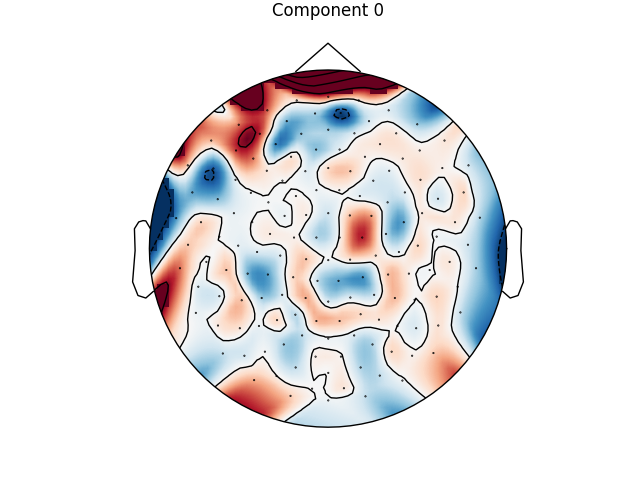
\includegraphics[width=\linewidth]{viz/max_scnn_raw/spatial_conv_1/component_0.png}\end{minipage}
\hspace*{\fill}
\begin{minipage}{0.31\textwidth}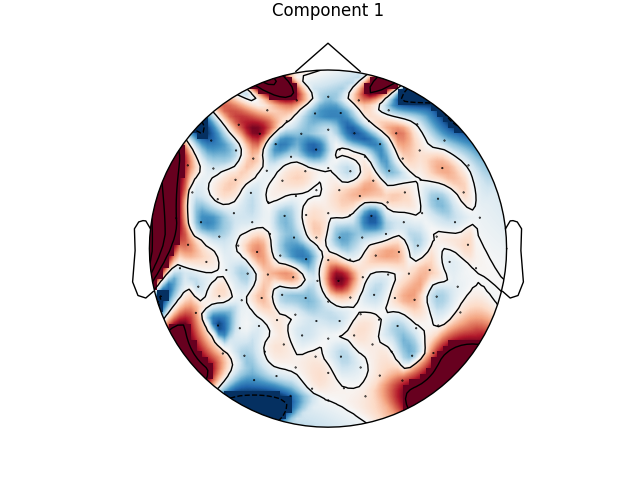
\includegraphics[width=\linewidth]{viz/max_scnn_raw/spatial_conv_1/component_1.png}\end{minipage}
\hspace*{\fill}
\begin{minipage}{0.31\textwidth}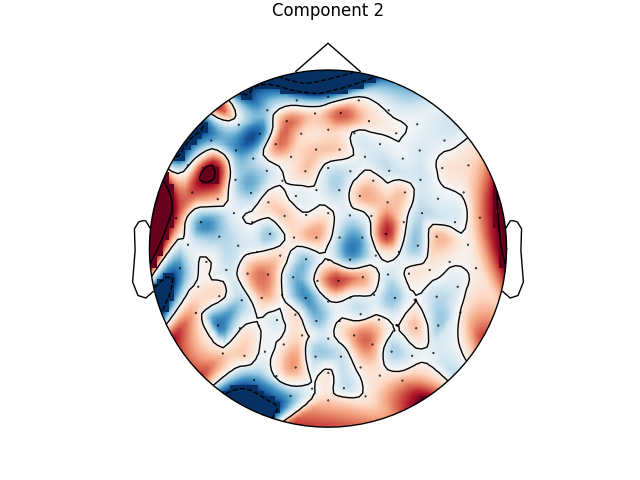
\includegraphics[width=\linewidth]{viz/max_scnn_raw/spatial_conv_1/component_2.png}\end{minipage}
\begin{minipage}{0.31\textwidth}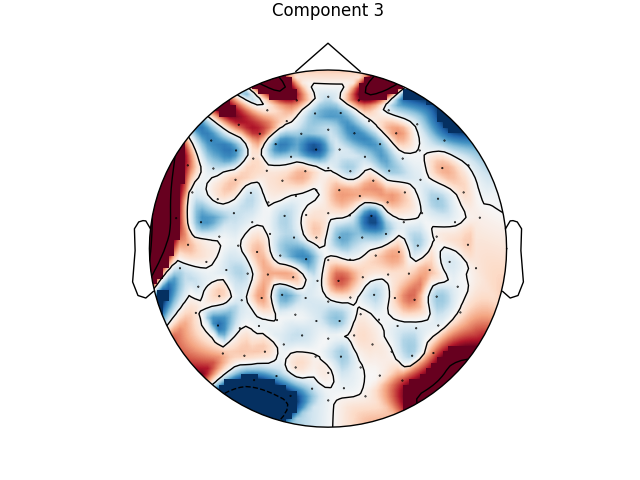
\includegraphics[width=\linewidth]{viz/max_scnn_raw/spatial_conv_1/component_3.png}\end{minipage}
\hspace*{\fill}
\begin{minipage}{0.31\textwidth}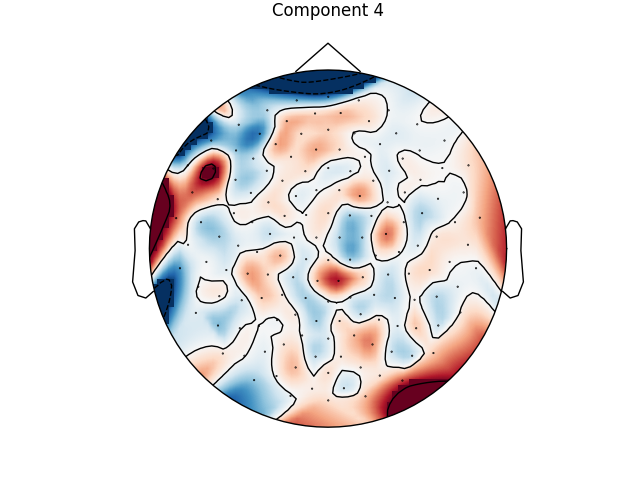
\includegraphics[width=\linewidth]{viz/max_scnn_raw/spatial_conv_1/component_4.png}\end{minipage}
\hspace*{\fill}
\begin{minipage}{0.31\textwidth}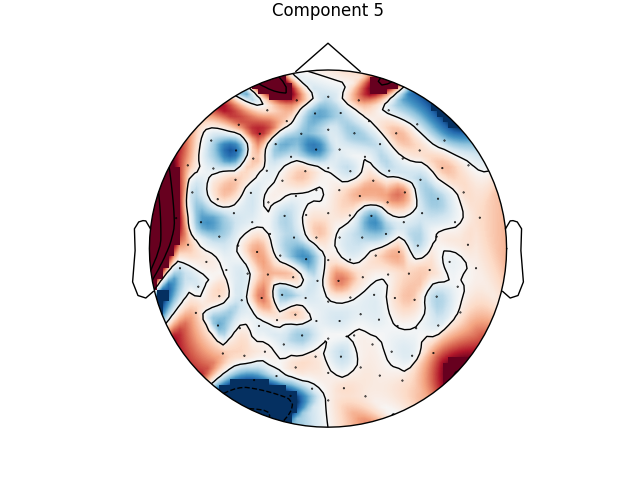
\includegraphics[width=\linewidth]{viz/max_scnn_raw/spatial_conv_1/component_5.png}\end{minipage}
\hspace*{\fill}
\vskip\baselineskip

\begin{minipage}{0.31\textwidth}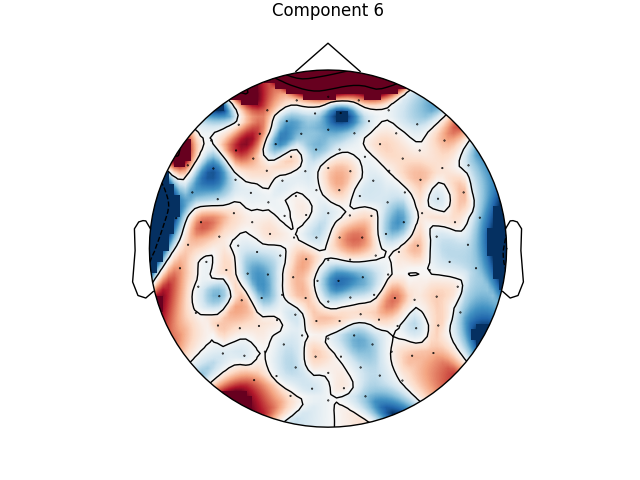
\includegraphics[width=\linewidth]{viz/max_scnn_raw/spatial_conv_1/component_6.png}\end{minipage}
\hspace*{\fill}
\begin{minipage}{0.31\textwidth}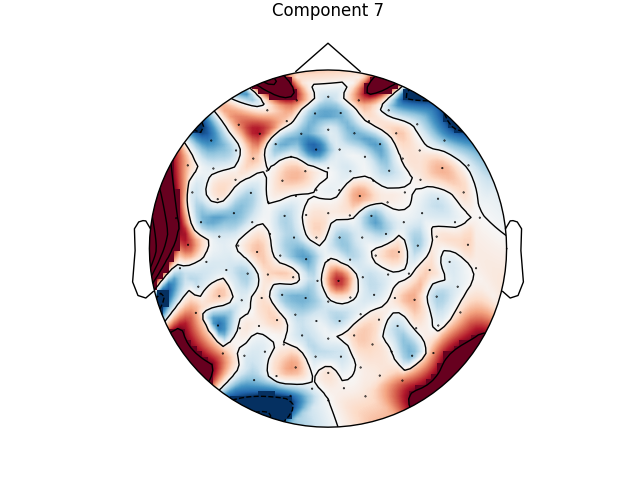
\includegraphics[width=\linewidth]{viz/max_scnn_raw/spatial_conv_1/component_7.png}\end{minipage}
\hspace*{\fill}
\begin{minipage}{0.31\textwidth}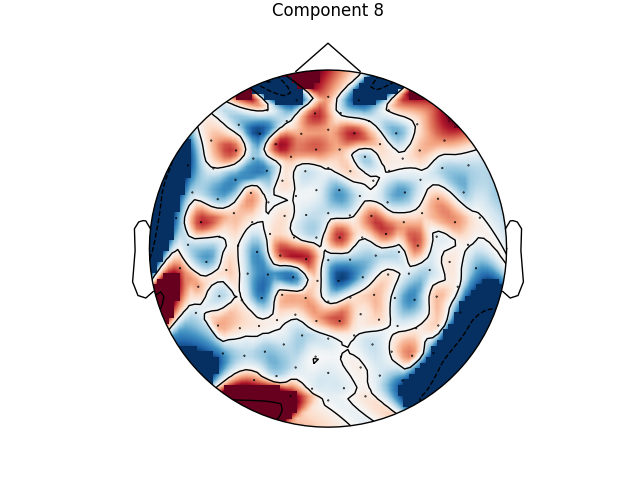
\includegraphics[width=\linewidth]{viz/max_scnn_raw/spatial_conv_1/component_8.png}\end{minipage}
%\hspace*{\fill}
%\vskip\baselineskip
\end{figure}

\begin{figure}

\begin{minipage}{0.31\textwidth}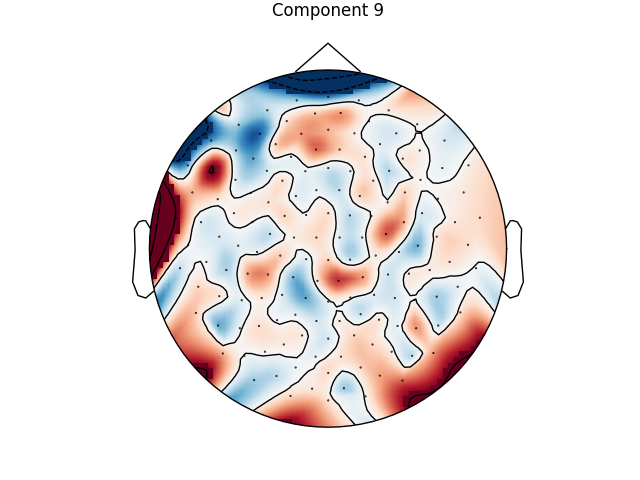
\includegraphics[width=\linewidth]{viz/max_scnn_raw/spatial_conv_1/component_9.png}\end{minipage}
\hspace*{\fill}
\begin{minipage}{0.31\textwidth}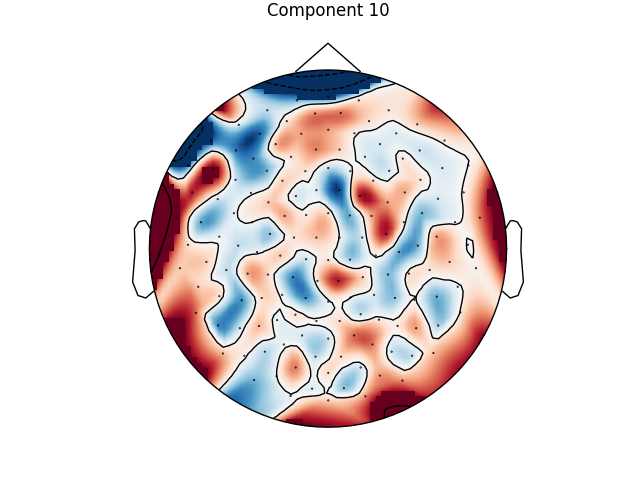
\includegraphics[width=\linewidth]{viz/max_scnn_raw/spatial_conv_1/component_10.png}\end{minipage}
\hspace*{\fill}
\begin{minipage}{0.31\textwidth}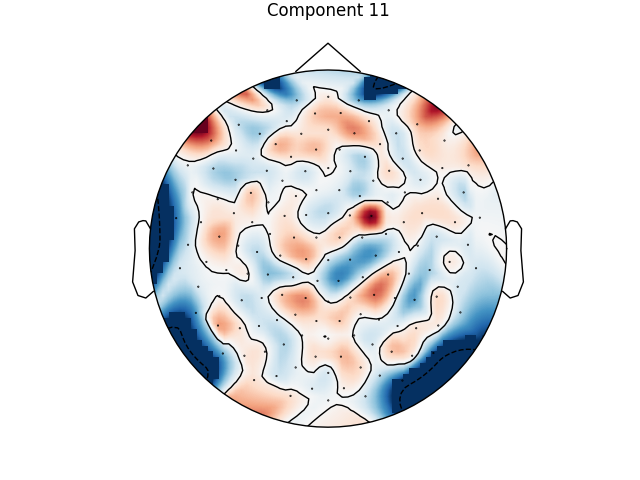
\includegraphics[width=\linewidth]{viz/max_scnn_raw/spatial_conv_1/component_11.png}\end{minipage}
\hspace*{\fill}
\vskip\baselineskip
\begin{minipage}{0.31\textwidth}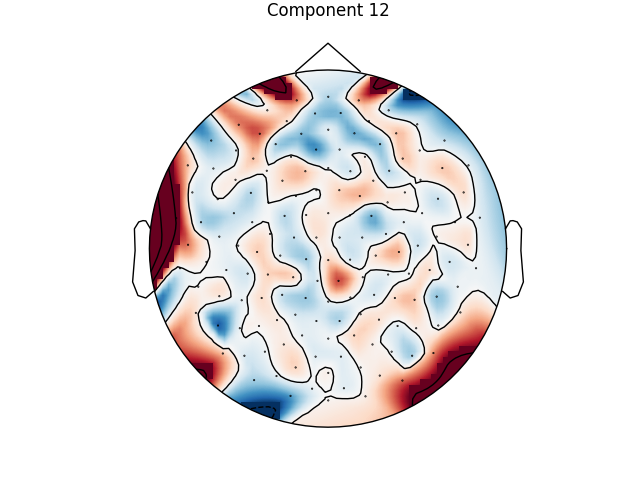
\includegraphics[width=\linewidth]{viz/max_scnn_raw/spatial_conv_1/component_12.png}\end{minipage}
\hspace*{\fill}
\begin{minipage}{0.31\textwidth}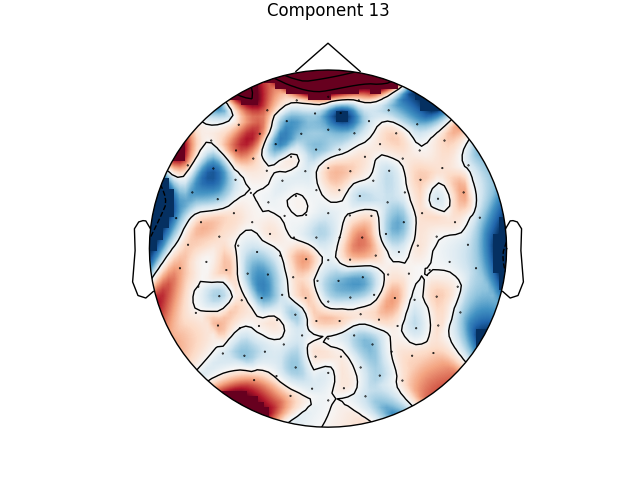
\includegraphics[width=\linewidth]{viz/max_scnn_raw/spatial_conv_1/component_13.png}\end{minipage}
\hspace*{\fill}
\begin{minipage}{0.31\textwidth}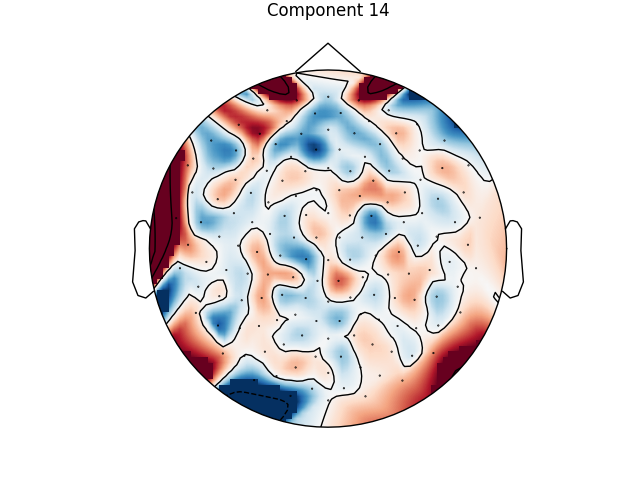
\includegraphics[width=\linewidth]{viz/max_scnn_raw/spatial_conv_1/component_14.png}\end{minipage}
\hspace*{\fill}
\vskip\baselineskip
\begin{minipage}{0.31\textwidth}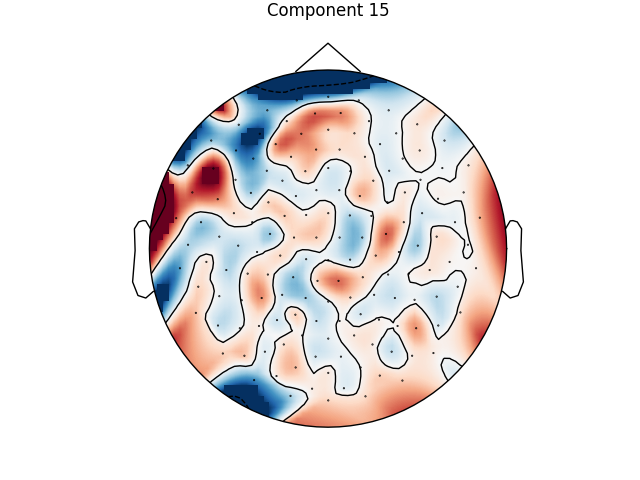
\includegraphics[width=\linewidth]{viz/max_scnn_raw/spatial_conv_1/component_15.png}\end{minipage}
\hspace*{\fill}
\begin{minipage}{0.31\textwidth}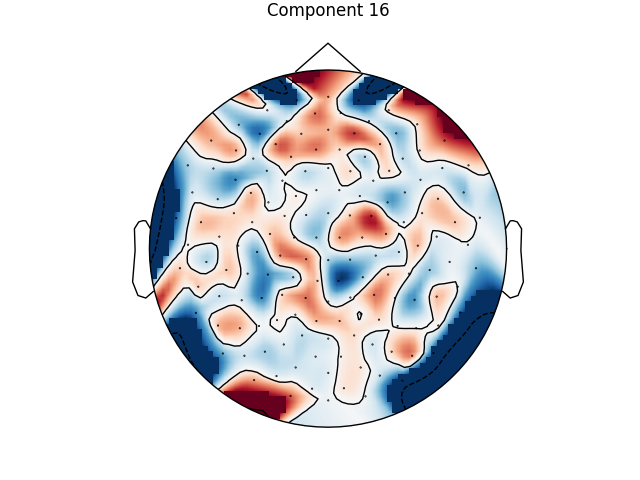
\includegraphics[width=\linewidth]{viz/max_scnn_raw/spatial_conv_1/component_16.png}\end{minipage}
\hspace*{\fill}
\begin{minipage}{0.31\textwidth}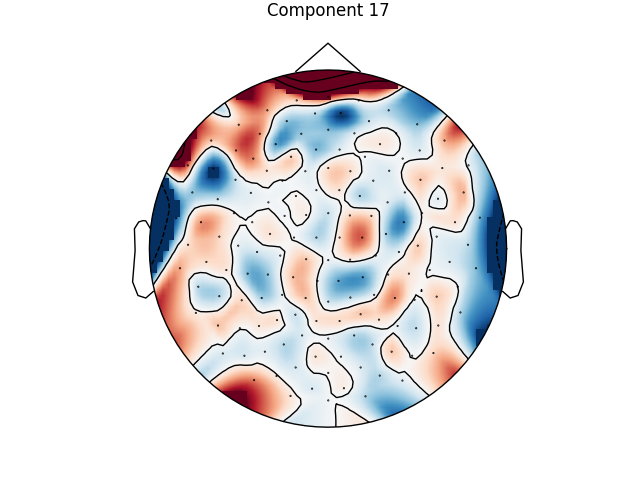
\includegraphics[width=\linewidth]{viz/max_scnn_raw/spatial_conv_1/component_17.png}\end{minipage}
\end{figure}

\begin{figure}
\begin{minipage}{0.31\textwidth}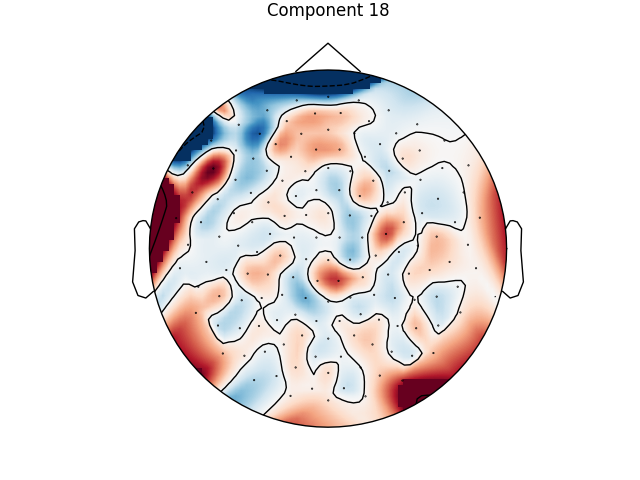
\includegraphics[width=\linewidth]{viz/max_scnn_raw/spatial_conv_1/component_18.png}\end{minipage}
\hspace*{\fill}
\begin{minipage}{0.31\textwidth}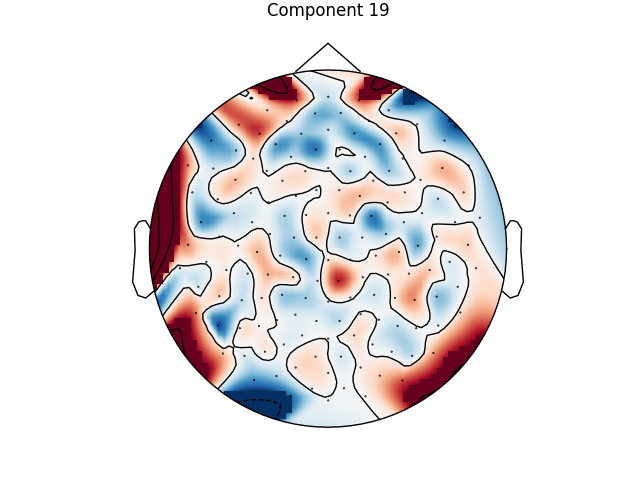
\includegraphics[width=\linewidth]{viz/max_scnn_raw/spatial_conv_1/component_19.png}\end{minipage}
\hspace*{\fill}
\begin{minipage}{0.31\textwidth}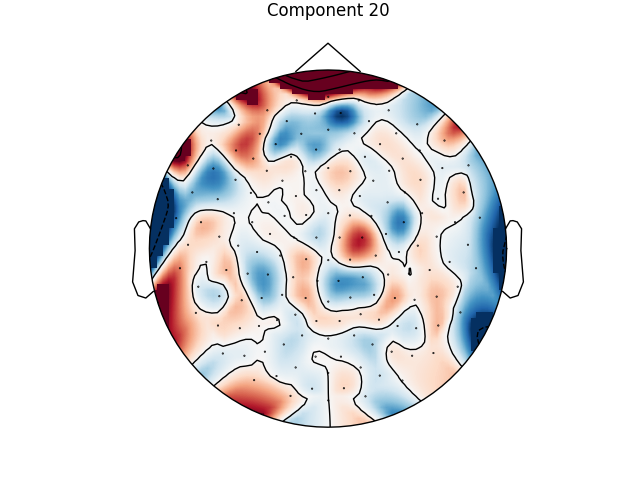
\includegraphics[width=\linewidth]{viz/max_scnn_raw/spatial_conv_1/component_20.png}\end{minipage}
\hspace*{\fill}
\vskip\baselineskip
\begin{minipage}{0.31\textwidth}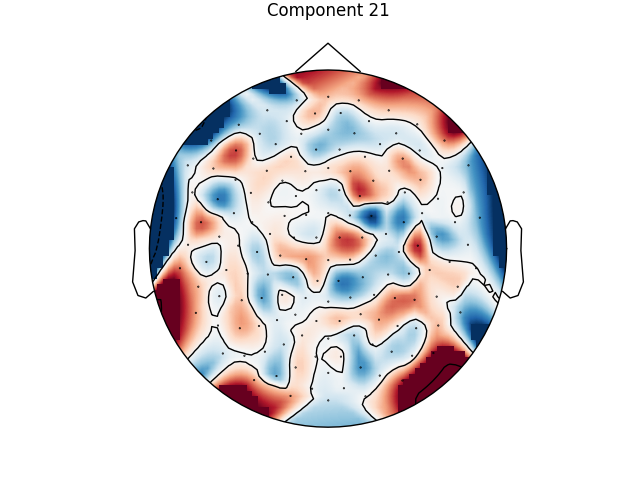
\includegraphics[width=\linewidth]{viz/max_scnn_raw/spatial_conv_1/component_21.png}\end{minipage}
\hspace*{\fill}
\begin{minipage}{0.31\textwidth}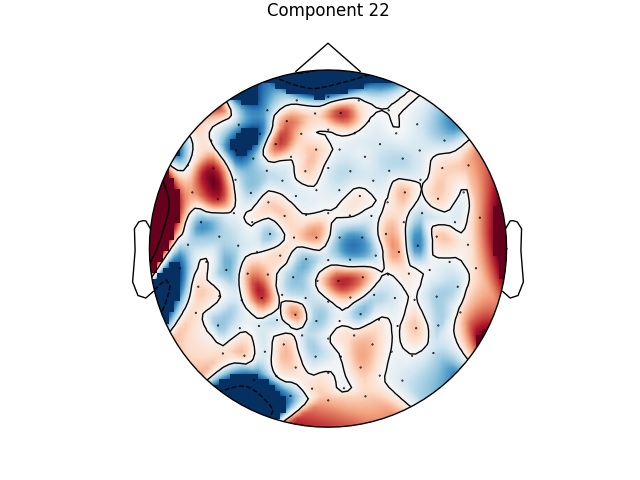
\includegraphics[width=\linewidth]{viz/max_scnn_raw/spatial_conv_1/component_22.png}\end{minipage}
\hspace*{\fill}
\begin{minipage}{0.31\textwidth}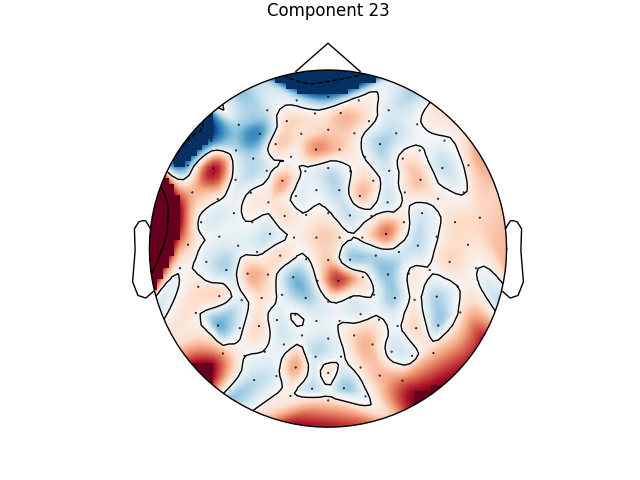
\includegraphics[width=\linewidth]{viz/max_scnn_raw/spatial_conv_1/component_23.png}\end{minipage}
\hspace*{\fill}
\vskip\baselineskip
\begin{minipage}{0.31\textwidth}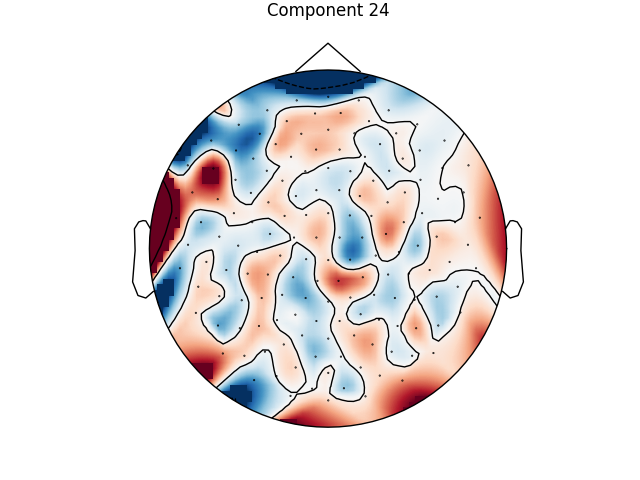
\includegraphics[width=\linewidth]{viz/max_scnn_raw/spatial_conv_1/component_24.png}\end{minipage}
\hspace*{\fill}
\begin{minipage}{0.31\textwidth}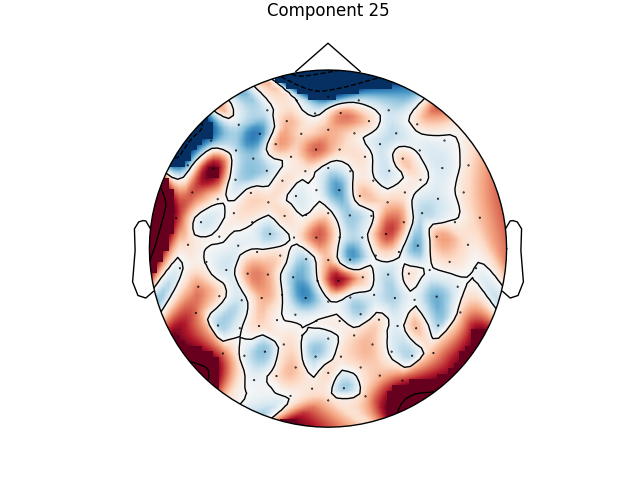
\includegraphics[width=\linewidth]{viz/max_scnn_raw/spatial_conv_1/component_25.png}\end{minipage}
\hspace*{\fill}
\begin{minipage}{0.31\textwidth}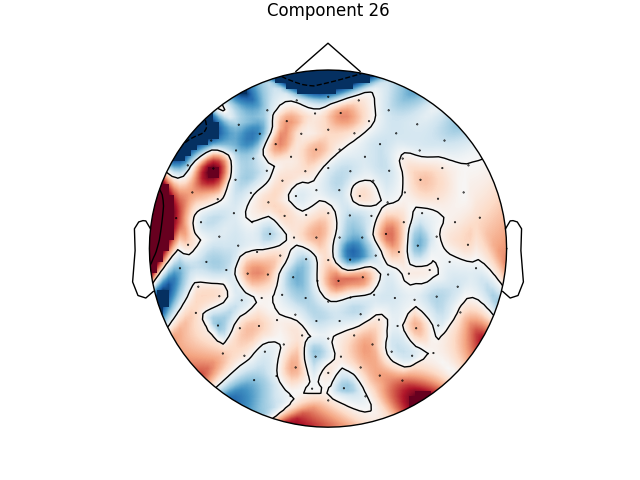
\includegraphics[width=\linewidth]{viz/max_scnn_raw/spatial_conv_1/component_26.png}\end{minipage}
\hspace*{\fill}
\vskip\baselineskip
\begin{minipage}{0.31\textwidth}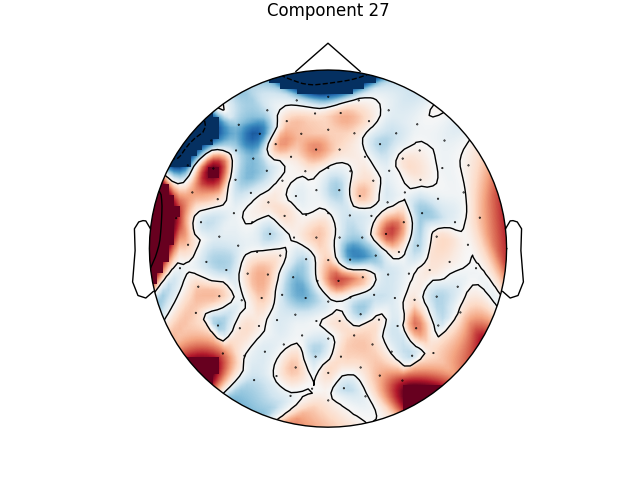
\includegraphics[width=\linewidth]{viz/max_scnn_raw/spatial_conv_1/component_27.png}\end{minipage}
\hspace*{\fill}
\begin{minipage}{0.31\textwidth}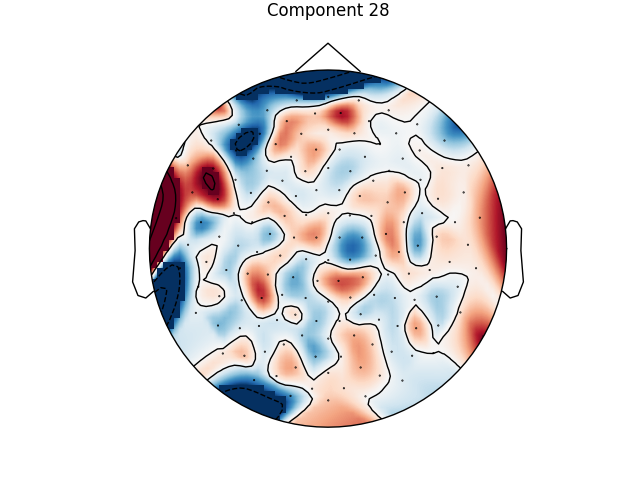
\includegraphics[width=\linewidth]{viz/max_scnn_raw/spatial_conv_1/component_28.png}\end{minipage}
\hspace*{\fill}
\begin{minipage}{0.31\textwidth}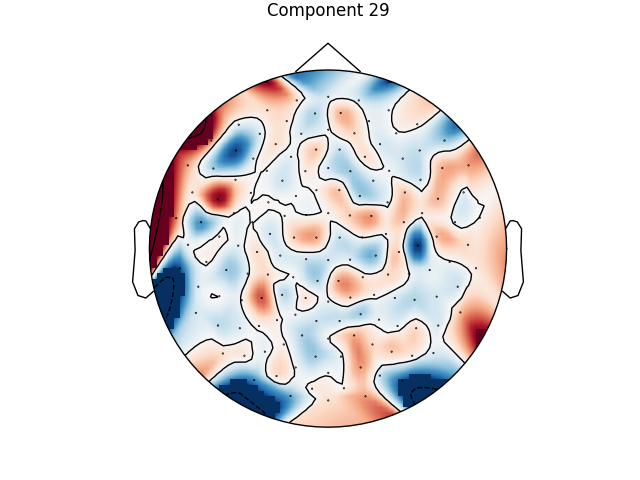
\includegraphics[width=\linewidth]{viz/max_scnn_raw/spatial_conv_1/component_29.png}\end{minipage}
\hspace*{\fill}
\vskip\baselineskip
\begin{minipage}{0.31\textwidth}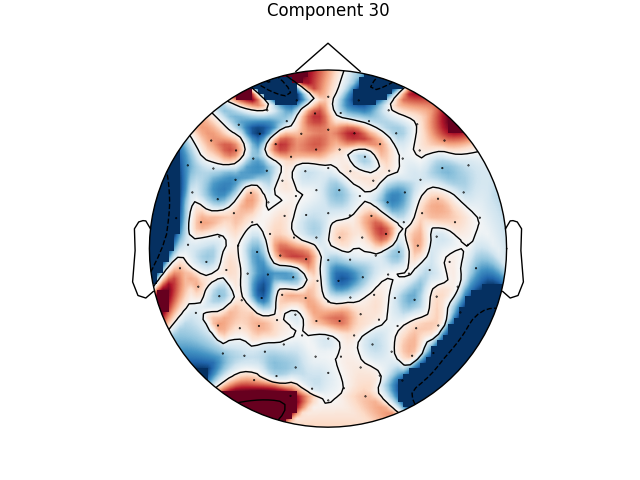
\includegraphics[width=\linewidth]{viz/max_scnn_raw/spatial_conv_1/component_30.png}\end{minipage}
\hspace*{\fill}
\begin{minipage}{0.31\textwidth}\includegraphics[width=\linewidth]{viz/max_scnn_raw/spatial_conv_1/component_31.png}\end{minipage}
\hspace*{\fill}
\begin{minipage}{0.31\textwidth}\includegraphics[width=\linewidth]{viz/max_scnn_raw/spatial_conv_1/component_32.png}\end{minipage}
\hspace*{\fill}
\vskip\baselineskip
\begin{minipage}{0.31\textwidth}\includegraphics[width=\linewidth]{viz/max_scnn_raw/spatial_conv_1/component_33.png}\end{minipage}
\hspace*{\fill}
\begin{minipage}{0.31\textwidth}\includegraphics[width=\linewidth]{viz/max_scnn_raw/spatial_conv_1/component_34.png}\end{minipage}
\hspace*{\fill}
\begin{minipage}{0.31\textwidth}\includegraphics[width=\linewidth]{viz/max_scnn_raw/spatial_conv_1/component_35.png}\end{minipage}
\end{figure}

\begin{figure}
\begin{minipage}{0.31\textwidth}\includegraphics[width=\linewidth]{viz/max_scnn_raw/spatial_conv_1/component_36.png}\end{minipage}
\hspace*{\fill}
\begin{minipage}{0.31\textwidth}\includegraphics[width=\linewidth]{viz/max_scnn_raw/spatial_conv_1/component_37.png}\end{minipage}
\hspace*{\fill}
\begin{minipage}{0.31\textwidth}\includegraphics[width=\linewidth]{viz/max_scnn_raw/spatial_conv_1/component_38.png}\end{minipage}
\hspace*{\fill}
\vskip\baselineskip
\begin{minipage}{0.31\textwidth}\includegraphics[width=\linewidth]{viz/max_scnn_raw/spatial_conv_1/component_39.png}\end{minipage}
\hspace*{\fill}
\begin{minipage}{0.31\textwidth}\includegraphics[width=\linewidth]{viz/max_scnn_raw/spatial_conv_1/component_40.png}\end{minipage}
\hspace*{\fill}
\begin{minipage}{0.31\textwidth}\includegraphics[width=\linewidth]{viz/max_scnn_raw/spatial_conv_1/component_41.png}\end{minipage}
\hspace*{\fill}
\vskip\baselineskip
\begin{minipage}{0.31\textwidth}\includegraphics[width=\linewidth]{viz/max_scnn_raw/spatial_conv_1/component_42.png}\end{minipage}
\hspace*{\fill}
\begin{minipage}{0.31\textwidth}\includegraphics[width=\linewidth]{viz/max_scnn_raw/spatial_conv_1/component_43.png}\end{minipage}
\hspace*{\fill}
\begin{minipage}{0.31\textwidth}\includegraphics[width=\linewidth]{viz/max_scnn_raw/spatial_conv_1/component_44.png}\end{minipage}
\hspace*{\fill}
\vskip\baselineskip
\begin{minipage}{0.31\textwidth}\includegraphics[width=\linewidth]{viz/max_scnn_raw/spatial_conv_1/component_45.png}\end{minipage}
\hspace*{\fill}
\begin{minipage}{0.31\textwidth}\includegraphics[width=\linewidth]{viz/max_scnn_raw/spatial_conv_1/component_46.png}\end{minipage}
\hspace*{\fill}
\begin{minipage}{0.31\textwidth}\includegraphics[width=\linewidth]{viz/max_scnn_raw/spatial_conv_1/component_47.png}\end{minipage}
\hspace*{\fill}
\vskip\baselineskip
\begin{minipage}{0.31\textwidth}\includegraphics[width=\linewidth]{viz/max_scnn_raw/spatial_conv_1/component_48.png}\end{minipage}
\hspace*{\fill}
\begin{minipage}{0.31\textwidth}\includegraphics[width=\linewidth]{viz/max_scnn_raw/spatial_conv_1/component_49.png}\end{minipage}
\hspace*{\fill}
\begin{minipage}{0.31\textwidth}\includegraphics[width=\linewidth]{viz/max_scnn_raw/spatial_conv_1/component_50.png}\end{minipage}
\hspace*{\fill}
\vskip\baselineskip
\begin{minipage}{0.31\textwidth}\includegraphics[width=\linewidth]{viz/max_scnn_raw/spatial_conv_1/component_51.png}\end{minipage}
\hspace*{\fill}
\begin{minipage}{0.31\textwidth}\includegraphics[width=\linewidth]{viz/max_scnn_raw/spatial_conv_1/component_52.png}\end{minipage}
\hspace*{\fill}
\begin{minipage}{0.31\textwidth}\includegraphics[width=\linewidth]{viz/max_scnn_raw/spatial_conv_1/component_53.png}\end{minipage}
\end{figure}

\begin{figure}
\begin{minipage}{0.31\textwidth}\includegraphics[width=\linewidth]{viz/max_scnn_raw/spatial_conv_1/component_54.png}\end{minipage}
\hspace*{\fill}
\begin{minipage}{0.31\textwidth}\includegraphics[width=\linewidth]{viz/max_scnn_raw/spatial_conv_1/component_55.png}\end{minipage}
\hspace*{\fill}
\begin{minipage}{0.31\textwidth}\includegraphics[width=\linewidth]{viz/max_scnn_raw/spatial_conv_1/component_56.png}\end{minipage}
\hspace*{\fill}
\vskip\baselineskip
\begin{minipage}{0.31\textwidth}\includegraphics[width=\linewidth]{viz/max_scnn_raw/spatial_conv_1/component_57.png}\end{minipage}
\hspace*{\fill}
\begin{minipage}{0.31\textwidth}\includegraphics[width=\linewidth]{viz/max_scnn_raw/spatial_conv_1/component_58.png}\end{minipage}
\hspace*{\fill}
\begin{minipage}{0.31\textwidth}\includegraphics[width=\linewidth]{viz/max_scnn_raw/spatial_conv_1/component_59.png}\end{minipage}
  
\end{figure}


\section{Ideal Spectrograms For Components}

Here, the left side represents the artificially generated data, and the right represents the high confience points.

% for i in range(60):
%         for j in range(2):
%             print("\\begin{{minipage}}{{0.45\\textwidth}}\\includegraphics[width=\\linewidth]{{viz/max_scnn_raw/OUT/class_{0}/component_{1}.png}}\\end{{minipage}}".format(j,i))
%             print("\\hspace*{\\fill}")
%             print("\\begin{{minipage}}{{0.45\\textwidth}}\\includegraphics[width=\\linewidth]{{viz/real_scnn_raw/OUT/class_{0}/component_{1}.png}}\\end{{minipage}}".format(j,i))
%             print("\\vskip\\baselineskip")
%         if (i + 1)  % 2 == 0:
%             print("\\end{figure}")
%             print("")
%             print("\\begin{figure}")


\begin{figure}

  \begin{minipage}{0.45\textwidth}\includegraphics[width=\linewidth]{viz/max_scnn_raw/OUT/class_0/component_0.png}\end{minipage}
\hspace*{\fill}
\begin{minipage}{0.45\textwidth}\includegraphics[width=\linewidth]{viz/real_scnn_raw/OUT/class_0/component_0.png}\end{minipage}
\vskip\baselineskip
\begin{minipage}{0.45\textwidth}\includegraphics[width=\linewidth]{viz/max_scnn_raw/OUT/class_1/component_0.png}\end{minipage}
\hspace*{\fill}
\begin{minipage}{0.45\textwidth}\includegraphics[width=\linewidth]{viz/real_scnn_raw/OUT/class_1/component_0.png}\end{minipage}
\vskip\baselineskip
\begin{minipage}{0.45\textwidth}\includegraphics[width=\linewidth]{viz/max_scnn_raw/OUT/class_0/component_1.png}\end{minipage}
\hspace*{\fill}
\begin{minipage}{0.45\textwidth}\includegraphics[width=\linewidth]{viz/real_scnn_raw/OUT/class_0/component_1.png}\end{minipage}
\vskip\baselineskip
\begin{minipage}{0.45\textwidth}\includegraphics[width=\linewidth]{viz/max_scnn_raw/OUT/class_1/component_1.png}\end{minipage}
\hspace*{\fill}
\begin{minipage}{0.45\textwidth}\includegraphics[width=\linewidth]{viz/real_scnn_raw/OUT/class_1/component_1.png}\end{minipage}
\vskip\baselineskip
\end{figure}

\begin{figure}
\begin{minipage}{0.45\textwidth}\includegraphics[width=\linewidth]{viz/max_scnn_raw/OUT/class_0/component_2.png}\end{minipage}
\hspace*{\fill}
\begin{minipage}{0.45\textwidth}\includegraphics[width=\linewidth]{viz/real_scnn_raw/OUT/class_0/component_2.png}\end{minipage}
\vskip\baselineskip
\begin{minipage}{0.45\textwidth}\includegraphics[width=\linewidth]{viz/max_scnn_raw/OUT/class_1/component_2.png}\end{minipage}
\hspace*{\fill}
\begin{minipage}{0.45\textwidth}\includegraphics[width=\linewidth]{viz/real_scnn_raw/OUT/class_1/component_2.png}\end{minipage}
\vskip\baselineskip
\begin{minipage}{0.45\textwidth}\includegraphics[width=\linewidth]{viz/max_scnn_raw/OUT/class_0/component_3.png}\end{minipage}
\hspace*{\fill}
\begin{minipage}{0.45\textwidth}\includegraphics[width=\linewidth]{viz/real_scnn_raw/OUT/class_0/component_3.png}\end{minipage}
\vskip\baselineskip
\begin{minipage}{0.45\textwidth}\includegraphics[width=\linewidth]{viz/max_scnn_raw/OUT/class_1/component_3.png}\end{minipage}
\hspace*{\fill}
\begin{minipage}{0.45\textwidth}\includegraphics[width=\linewidth]{viz/real_scnn_raw/OUT/class_1/component_3.png}\end{minipage}
\vskip\baselineskip
\end{figure}

\begin{figure}
\begin{minipage}{0.45\textwidth}\includegraphics[width=\linewidth]{viz/max_scnn_raw/OUT/class_0/component_4.png}\end{minipage}
\hspace*{\fill}
\begin{minipage}{0.45\textwidth}\includegraphics[width=\linewidth]{viz/real_scnn_raw/OUT/class_0/component_4.png}\end{minipage}
\vskip\baselineskip
\begin{minipage}{0.45\textwidth}\includegraphics[width=\linewidth]{viz/max_scnn_raw/OUT/class_1/component_4.png}\end{minipage}
\hspace*{\fill}
\begin{minipage}{0.45\textwidth}\includegraphics[width=\linewidth]{viz/real_scnn_raw/OUT/class_1/component_4.png}\end{minipage}
\vskip\baselineskip
\begin{minipage}{0.45\textwidth}\includegraphics[width=\linewidth]{viz/max_scnn_raw/OUT/class_0/component_5.png}\end{minipage}
\hspace*{\fill}
\begin{minipage}{0.45\textwidth}\includegraphics[width=\linewidth]{viz/real_scnn_raw/OUT/class_0/component_5.png}\end{minipage}
\vskip\baselineskip
\begin{minipage}{0.45\textwidth}\includegraphics[width=\linewidth]{viz/max_scnn_raw/OUT/class_1/component_5.png}\end{minipage}
\hspace*{\fill}
\begin{minipage}{0.45\textwidth}\includegraphics[width=\linewidth]{viz/real_scnn_raw/OUT/class_1/component_5.png}\end{minipage}
\vskip\baselineskip
\end{figure}

\begin{figure}
\begin{minipage}{0.45\textwidth}\includegraphics[width=\linewidth]{viz/max_scnn_raw/OUT/class_0/component_6.png}\end{minipage}
\hspace*{\fill}
\begin{minipage}{0.45\textwidth}\includegraphics[width=\linewidth]{viz/real_scnn_raw/OUT/class_0/component_6.png}\end{minipage}
\vskip\baselineskip
\begin{minipage}{0.45\textwidth}\includegraphics[width=\linewidth]{viz/max_scnn_raw/OUT/class_1/component_6.png}\end{minipage}
\hspace*{\fill}
\begin{minipage}{0.45\textwidth}\includegraphics[width=\linewidth]{viz/real_scnn_raw/OUT/class_1/component_6.png}\end{minipage}
\vskip\baselineskip
\begin{minipage}{0.45\textwidth}\includegraphics[width=\linewidth]{viz/max_scnn_raw/OUT/class_0/component_7.png}\end{minipage}
\hspace*{\fill}
\begin{minipage}{0.45\textwidth}\includegraphics[width=\linewidth]{viz/real_scnn_raw/OUT/class_0/component_7.png}\end{minipage}
\vskip\baselineskip
\begin{minipage}{0.45\textwidth}\includegraphics[width=\linewidth]{viz/max_scnn_raw/OUT/class_1/component_7.png}\end{minipage}
\hspace*{\fill}
\begin{minipage}{0.45\textwidth}\includegraphics[width=\linewidth]{viz/real_scnn_raw/OUT/class_1/component_7.png}\end{minipage}
\vskip\baselineskip
\end{figure}

\begin{figure}
\begin{minipage}{0.45\textwidth}\includegraphics[width=\linewidth]{viz/max_scnn_raw/OUT/class_0/component_8.png}\end{minipage}
\hspace*{\fill}
\begin{minipage}{0.45\textwidth}\includegraphics[width=\linewidth]{viz/real_scnn_raw/OUT/class_0/component_8.png}\end{minipage}
\vskip\baselineskip
\begin{minipage}{0.45\textwidth}\includegraphics[width=\linewidth]{viz/max_scnn_raw/OUT/class_1/component_8.png}\end{minipage}
\hspace*{\fill}
\begin{minipage}{0.45\textwidth}\includegraphics[width=\linewidth]{viz/real_scnn_raw/OUT/class_1/component_8.png}\end{minipage}
\vskip\baselineskip
\begin{minipage}{0.45\textwidth}\includegraphics[width=\linewidth]{viz/max_scnn_raw/OUT/class_0/component_9.png}\end{minipage}
\hspace*{\fill}
\begin{minipage}{0.45\textwidth}\includegraphics[width=\linewidth]{viz/real_scnn_raw/OUT/class_0/component_9.png}\end{minipage}
\vskip\baselineskip
\begin{minipage}{0.45\textwidth}\includegraphics[width=\linewidth]{viz/max_scnn_raw/OUT/class_1/component_9.png}\end{minipage}
\hspace*{\fill}
\begin{minipage}{0.45\textwidth}\includegraphics[width=\linewidth]{viz/real_scnn_raw/OUT/class_1/component_9.png}\end{minipage}
\vskip\baselineskip
\end{figure}

\begin{figure}
\begin{minipage}{0.45\textwidth}\includegraphics[width=\linewidth]{viz/max_scnn_raw/OUT/class_0/component_10.png}\end{minipage}
\hspace*{\fill}
\begin{minipage}{0.45\textwidth}\includegraphics[width=\linewidth]{viz/real_scnn_raw/OUT/class_0/component_10.png}\end{minipage}
\vskip\baselineskip
\begin{minipage}{0.45\textwidth}\includegraphics[width=\linewidth]{viz/max_scnn_raw/OUT/class_1/component_10.png}\end{minipage}
\hspace*{\fill}
\begin{minipage}{0.45\textwidth}\includegraphics[width=\linewidth]{viz/real_scnn_raw/OUT/class_1/component_10.png}\end{minipage}
\vskip\baselineskip
\begin{minipage}{0.45\textwidth}\includegraphics[width=\linewidth]{viz/max_scnn_raw/OUT/class_0/component_11.png}\end{minipage}
\hspace*{\fill}
\begin{minipage}{0.45\textwidth}\includegraphics[width=\linewidth]{viz/real_scnn_raw/OUT/class_0/component_11.png}\end{minipage}
\vskip\baselineskip
\begin{minipage}{0.45\textwidth}\includegraphics[width=\linewidth]{viz/max_scnn_raw/OUT/class_1/component_11.png}\end{minipage}
\hspace*{\fill}
\begin{minipage}{0.45\textwidth}\includegraphics[width=\linewidth]{viz/real_scnn_raw/OUT/class_1/component_11.png}\end{minipage}
\vskip\baselineskip
\end{figure}

\begin{figure}
\begin{minipage}{0.45\textwidth}\includegraphics[width=\linewidth]{viz/max_scnn_raw/OUT/class_0/component_12.png}\end{minipage}
\hspace*{\fill}
\begin{minipage}{0.45\textwidth}\includegraphics[width=\linewidth]{viz/real_scnn_raw/OUT/class_0/component_12.png}\end{minipage}
\vskip\baselineskip
\begin{minipage}{0.45\textwidth}\includegraphics[width=\linewidth]{viz/max_scnn_raw/OUT/class_1/component_12.png}\end{minipage}
\hspace*{\fill}
\begin{minipage}{0.45\textwidth}\includegraphics[width=\linewidth]{viz/real_scnn_raw/OUT/class_1/component_12.png}\end{minipage}
\vskip\baselineskip
\begin{minipage}{0.45\textwidth}\includegraphics[width=\linewidth]{viz/max_scnn_raw/OUT/class_0/component_13.png}\end{minipage}
\hspace*{\fill}
\begin{minipage}{0.45\textwidth}\includegraphics[width=\linewidth]{viz/real_scnn_raw/OUT/class_0/component_13.png}\end{minipage}
\vskip\baselineskip
\begin{minipage}{0.45\textwidth}\includegraphics[width=\linewidth]{viz/max_scnn_raw/OUT/class_1/component_13.png}\end{minipage}
\hspace*{\fill}
\begin{minipage}{0.45\textwidth}\includegraphics[width=\linewidth]{viz/real_scnn_raw/OUT/class_1/component_13.png}\end{minipage}
\vskip\baselineskip
\end{figure}

\begin{figure}
\begin{minipage}{0.45\textwidth}\includegraphics[width=\linewidth]{viz/max_scnn_raw/OUT/class_0/component_14.png}\end{minipage}
\hspace*{\fill}
\begin{minipage}{0.45\textwidth}\includegraphics[width=\linewidth]{viz/real_scnn_raw/OUT/class_0/component_14.png}\end{minipage}
\vskip\baselineskip
\begin{minipage}{0.45\textwidth}\includegraphics[width=\linewidth]{viz/max_scnn_raw/OUT/class_1/component_14.png}\end{minipage}
\hspace*{\fill}
\begin{minipage}{0.45\textwidth}\includegraphics[width=\linewidth]{viz/real_scnn_raw/OUT/class_1/component_14.png}\end{minipage}
\vskip\baselineskip
\begin{minipage}{0.45\textwidth}\includegraphics[width=\linewidth]{viz/max_scnn_raw/OUT/class_0/component_15.png}\end{minipage}
\hspace*{\fill}
\begin{minipage}{0.45\textwidth}\includegraphics[width=\linewidth]{viz/real_scnn_raw/OUT/class_0/component_15.png}\end{minipage}
\vskip\baselineskip
\begin{minipage}{0.45\textwidth}\includegraphics[width=\linewidth]{viz/max_scnn_raw/OUT/class_1/component_15.png}\end{minipage}
\hspace*{\fill}
\begin{minipage}{0.45\textwidth}\includegraphics[width=\linewidth]{viz/real_scnn_raw/OUT/class_1/component_15.png}\end{minipage}
\vskip\baselineskip
\end{figure}

\begin{figure}
\begin{minipage}{0.45\textwidth}\includegraphics[width=\linewidth]{viz/max_scnn_raw/OUT/class_0/component_16.png}\end{minipage}
\hspace*{\fill}
\begin{minipage}{0.45\textwidth}\includegraphics[width=\linewidth]{viz/real_scnn_raw/OUT/class_0/component_16.png}\end{minipage}
\vskip\baselineskip
\begin{minipage}{0.45\textwidth}\includegraphics[width=\linewidth]{viz/max_scnn_raw/OUT/class_1/component_16.png}\end{minipage}
\hspace*{\fill}
\begin{minipage}{0.45\textwidth}\includegraphics[width=\linewidth]{viz/real_scnn_raw/OUT/class_1/component_16.png}\end{minipage}
\vskip\baselineskip
\begin{minipage}{0.45\textwidth}\includegraphics[width=\linewidth]{viz/max_scnn_raw/OUT/class_0/component_17.png}\end{minipage}
\hspace*{\fill}
\begin{minipage}{0.45\textwidth}\includegraphics[width=\linewidth]{viz/real_scnn_raw/OUT/class_0/component_17.png}\end{minipage}
\vskip\baselineskip
\begin{minipage}{0.45\textwidth}\includegraphics[width=\linewidth]{viz/max_scnn_raw/OUT/class_1/component_17.png}\end{minipage}
\hspace*{\fill}
\begin{minipage}{0.45\textwidth}\includegraphics[width=\linewidth]{viz/real_scnn_raw/OUT/class_1/component_17.png}\end{minipage}
\vskip\baselineskip
\end{figure}

\begin{figure}
\begin{minipage}{0.45\textwidth}\includegraphics[width=\linewidth]{viz/max_scnn_raw/OUT/class_0/component_18.png}\end{minipage}
\hspace*{\fill}
\begin{minipage}{0.45\textwidth}\includegraphics[width=\linewidth]{viz/real_scnn_raw/OUT/class_0/component_18.png}\end{minipage}
\vskip\baselineskip
\begin{minipage}{0.45\textwidth}\includegraphics[width=\linewidth]{viz/max_scnn_raw/OUT/class_1/component_18.png}\end{minipage}
\hspace*{\fill}
\begin{minipage}{0.45\textwidth}\includegraphics[width=\linewidth]{viz/real_scnn_raw/OUT/class_1/component_18.png}\end{minipage}
\vskip\baselineskip
\begin{minipage}{0.45\textwidth}\includegraphics[width=\linewidth]{viz/max_scnn_raw/OUT/class_0/component_19.png}\end{minipage}
\hspace*{\fill}
\begin{minipage}{0.45\textwidth}\includegraphics[width=\linewidth]{viz/real_scnn_raw/OUT/class_0/component_19.png}\end{minipage}
\vskip\baselineskip
\begin{minipage}{0.45\textwidth}\includegraphics[width=\linewidth]{viz/max_scnn_raw/OUT/class_1/component_19.png}\end{minipage}
\hspace*{\fill}
\begin{minipage}{0.45\textwidth}\includegraphics[width=\linewidth]{viz/real_scnn_raw/OUT/class_1/component_19.png}\end{minipage}
\vskip\baselineskip
\end{figure}

\begin{figure}
\begin{minipage}{0.45\textwidth}\includegraphics[width=\linewidth]{viz/max_scnn_raw/OUT/class_0/component_20.png}\end{minipage}
\hspace*{\fill}
\begin{minipage}{0.45\textwidth}\includegraphics[width=\linewidth]{viz/real_scnn_raw/OUT/class_0/component_20.png}\end{minipage}
\vskip\baselineskip
\begin{minipage}{0.45\textwidth}\includegraphics[width=\linewidth]{viz/max_scnn_raw/OUT/class_1/component_20.png}\end{minipage}
\hspace*{\fill}
\begin{minipage}{0.45\textwidth}\includegraphics[width=\linewidth]{viz/real_scnn_raw/OUT/class_1/component_20.png}\end{minipage}
\vskip\baselineskip
\begin{minipage}{0.45\textwidth}\includegraphics[width=\linewidth]{viz/max_scnn_raw/OUT/class_0/component_21.png}\end{minipage}
\hspace*{\fill}
\begin{minipage}{0.45\textwidth}\includegraphics[width=\linewidth]{viz/real_scnn_raw/OUT/class_0/component_21.png}\end{minipage}
\vskip\baselineskip
\begin{minipage}{0.45\textwidth}\includegraphics[width=\linewidth]{viz/max_scnn_raw/OUT/class_1/component_21.png}\end{minipage}
\hspace*{\fill}
\begin{minipage}{0.45\textwidth}\includegraphics[width=\linewidth]{viz/real_scnn_raw/OUT/class_1/component_21.png}\end{minipage}
\vskip\baselineskip
\end{figure}

\begin{figure}
\begin{minipage}{0.45\textwidth}\includegraphics[width=\linewidth]{viz/max_scnn_raw/OUT/class_0/component_22.png}\end{minipage}
\hspace*{\fill}
\begin{minipage}{0.45\textwidth}\includegraphics[width=\linewidth]{viz/real_scnn_raw/OUT/class_0/component_22.png}\end{minipage}
\vskip\baselineskip
\begin{minipage}{0.45\textwidth}\includegraphics[width=\linewidth]{viz/max_scnn_raw/OUT/class_1/component_22.png}\end{minipage}
\hspace*{\fill}
\begin{minipage}{0.45\textwidth}\includegraphics[width=\linewidth]{viz/real_scnn_raw/OUT/class_1/component_22.png}\end{minipage}
\vskip\baselineskip
\begin{minipage}{0.45\textwidth}\includegraphics[width=\linewidth]{viz/max_scnn_raw/OUT/class_0/component_23.png}\end{minipage}
\hspace*{\fill}
\begin{minipage}{0.45\textwidth}\includegraphics[width=\linewidth]{viz/real_scnn_raw/OUT/class_0/component_23.png}\end{minipage}
\vskip\baselineskip
\begin{minipage}{0.45\textwidth}\includegraphics[width=\linewidth]{viz/max_scnn_raw/OUT/class_1/component_23.png}\end{minipage}
\hspace*{\fill}
\begin{minipage}{0.45\textwidth}\includegraphics[width=\linewidth]{viz/real_scnn_raw/OUT/class_1/component_23.png}\end{minipage}
\vskip\baselineskip
\end{figure}

\begin{figure}
\begin{minipage}{0.45\textwidth}\includegraphics[width=\linewidth]{viz/max_scnn_raw/OUT/class_0/component_24.png}\end{minipage}
\hspace*{\fill}
\begin{minipage}{0.45\textwidth}\includegraphics[width=\linewidth]{viz/real_scnn_raw/OUT/class_0/component_24.png}\end{minipage}
\vskip\baselineskip
\begin{minipage}{0.45\textwidth}\includegraphics[width=\linewidth]{viz/max_scnn_raw/OUT/class_1/component_24.png}\end{minipage}
\hspace*{\fill}
\begin{minipage}{0.45\textwidth}\includegraphics[width=\linewidth]{viz/real_scnn_raw/OUT/class_1/component_24.png}\end{minipage}
\vskip\baselineskip
\begin{minipage}{0.45\textwidth}\includegraphics[width=\linewidth]{viz/max_scnn_raw/OUT/class_0/component_25.png}\end{minipage}
\hspace*{\fill}
\begin{minipage}{0.45\textwidth}\includegraphics[width=\linewidth]{viz/real_scnn_raw/OUT/class_0/component_25.png}\end{minipage}
\vskip\baselineskip
\begin{minipage}{0.45\textwidth}\includegraphics[width=\linewidth]{viz/max_scnn_raw/OUT/class_1/component_25.png}\end{minipage}
\hspace*{\fill}
\begin{minipage}{0.45\textwidth}\includegraphics[width=\linewidth]{viz/real_scnn_raw/OUT/class_1/component_25.png}\end{minipage}
\vskip\baselineskip
\end{figure}

\begin{figure}
\begin{minipage}{0.45\textwidth}\includegraphics[width=\linewidth]{viz/max_scnn_raw/OUT/class_0/component_26.png}\end{minipage}
\hspace*{\fill}
\begin{minipage}{0.45\textwidth}\includegraphics[width=\linewidth]{viz/real_scnn_raw/OUT/class_0/component_26.png}\end{minipage}
\vskip\baselineskip
\begin{minipage}{0.45\textwidth}\includegraphics[width=\linewidth]{viz/max_scnn_raw/OUT/class_1/component_26.png}\end{minipage}
\hspace*{\fill}
\begin{minipage}{0.45\textwidth}\includegraphics[width=\linewidth]{viz/real_scnn_raw/OUT/class_1/component_26.png}\end{minipage}
\vskip\baselineskip
\begin{minipage}{0.45\textwidth}\includegraphics[width=\linewidth]{viz/max_scnn_raw/OUT/class_0/component_27.png}\end{minipage}
\hspace*{\fill}
\begin{minipage}{0.45\textwidth}\includegraphics[width=\linewidth]{viz/real_scnn_raw/OUT/class_0/component_27.png}\end{minipage}
\vskip\baselineskip
\begin{minipage}{0.45\textwidth}\includegraphics[width=\linewidth]{viz/max_scnn_raw/OUT/class_1/component_27.png}\end{minipage}
\hspace*{\fill}
\begin{minipage}{0.45\textwidth}\includegraphics[width=\linewidth]{viz/real_scnn_raw/OUT/class_1/component_27.png}\end{minipage}
\vskip\baselineskip
\end{figure}

\begin{figure}
\begin{minipage}{0.45\textwidth}\includegraphics[width=\linewidth]{viz/max_scnn_raw/OUT/class_0/component_28.png}\end{minipage}
\hspace*{\fill}
\begin{minipage}{0.45\textwidth}\includegraphics[width=\linewidth]{viz/real_scnn_raw/OUT/class_0/component_28.png}\end{minipage}
\vskip\baselineskip
\begin{minipage}{0.45\textwidth}\includegraphics[width=\linewidth]{viz/max_scnn_raw/OUT/class_1/component_28.png}\end{minipage}
\hspace*{\fill}
\begin{minipage}{0.45\textwidth}\includegraphics[width=\linewidth]{viz/real_scnn_raw/OUT/class_1/component_28.png}\end{minipage}
\vskip\baselineskip
\begin{minipage}{0.45\textwidth}\includegraphics[width=\linewidth]{viz/max_scnn_raw/OUT/class_0/component_29.png}\end{minipage}
\hspace*{\fill}
\begin{minipage}{0.45\textwidth}\includegraphics[width=\linewidth]{viz/real_scnn_raw/OUT/class_0/component_29.png}\end{minipage}
\vskip\baselineskip
\begin{minipage}{0.45\textwidth}\includegraphics[width=\linewidth]{viz/max_scnn_raw/OUT/class_1/component_29.png}\end{minipage}
\hspace*{\fill}
\begin{minipage}{0.45\textwidth}\includegraphics[width=\linewidth]{viz/real_scnn_raw/OUT/class_1/component_29.png}\end{minipage}
\vskip\baselineskip
\end{figure}

\begin{figure}
\begin{minipage}{0.45\textwidth}\includegraphics[width=\linewidth]{viz/max_scnn_raw/OUT/class_0/component_30.png}\end{minipage}
\hspace*{\fill}
\begin{minipage}{0.45\textwidth}\includegraphics[width=\linewidth]{viz/real_scnn_raw/OUT/class_0/component_30.png}\end{minipage}
\vskip\baselineskip
\begin{minipage}{0.45\textwidth}\includegraphics[width=\linewidth]{viz/max_scnn_raw/OUT/class_1/component_30.png}\end{minipage}
\hspace*{\fill}
\begin{minipage}{0.45\textwidth}\includegraphics[width=\linewidth]{viz/real_scnn_raw/OUT/class_1/component_30.png}\end{minipage}
\vskip\baselineskip
\begin{minipage}{0.45\textwidth}\includegraphics[width=\linewidth]{viz/max_scnn_raw/OUT/class_0/component_31.png}\end{minipage}
\hspace*{\fill}
\begin{minipage}{0.45\textwidth}\includegraphics[width=\linewidth]{viz/real_scnn_raw/OUT/class_0/component_31.png}\end{minipage}
\vskip\baselineskip
\begin{minipage}{0.45\textwidth}\includegraphics[width=\linewidth]{viz/max_scnn_raw/OUT/class_1/component_31.png}\end{minipage}
\hspace*{\fill}
\begin{minipage}{0.45\textwidth}\includegraphics[width=\linewidth]{viz/real_scnn_raw/OUT/class_1/component_31.png}\end{minipage}
\vskip\baselineskip
\end{figure}

\begin{figure}
\begin{minipage}{0.45\textwidth}\includegraphics[width=\linewidth]{viz/max_scnn_raw/OUT/class_0/component_32.png}\end{minipage}
\hspace*{\fill}
\begin{minipage}{0.45\textwidth}\includegraphics[width=\linewidth]{viz/real_scnn_raw/OUT/class_0/component_32.png}\end{minipage}
\vskip\baselineskip
\begin{minipage}{0.45\textwidth}\includegraphics[width=\linewidth]{viz/max_scnn_raw/OUT/class_1/component_32.png}\end{minipage}
\hspace*{\fill}
\begin{minipage}{0.45\textwidth}\includegraphics[width=\linewidth]{viz/real_scnn_raw/OUT/class_1/component_32.png}\end{minipage}
\vskip\baselineskip
\begin{minipage}{0.45\textwidth}\includegraphics[width=\linewidth]{viz/max_scnn_raw/OUT/class_0/component_33.png}\end{minipage}
\hspace*{\fill}
\begin{minipage}{0.45\textwidth}\includegraphics[width=\linewidth]{viz/real_scnn_raw/OUT/class_0/component_33.png}\end{minipage}
\vskip\baselineskip
\begin{minipage}{0.45\textwidth}\includegraphics[width=\linewidth]{viz/max_scnn_raw/OUT/class_1/component_33.png}\end{minipage}
\hspace*{\fill}
\begin{minipage}{0.45\textwidth}\includegraphics[width=\linewidth]{viz/real_scnn_raw/OUT/class_1/component_33.png}\end{minipage}
\vskip\baselineskip
\end{figure}

\begin{figure}
\begin{minipage}{0.45\textwidth}\includegraphics[width=\linewidth]{viz/max_scnn_raw/OUT/class_0/component_34.png}\end{minipage}
\hspace*{\fill}
\begin{minipage}{0.45\textwidth}\includegraphics[width=\linewidth]{viz/real_scnn_raw/OUT/class_0/component_34.png}\end{minipage}
\vskip\baselineskip
\begin{minipage}{0.45\textwidth}\includegraphics[width=\linewidth]{viz/max_scnn_raw/OUT/class_1/component_34.png}\end{minipage}
\hspace*{\fill}
\begin{minipage}{0.45\textwidth}\includegraphics[width=\linewidth]{viz/real_scnn_raw/OUT/class_1/component_34.png}\end{minipage}
\vskip\baselineskip
\begin{minipage}{0.45\textwidth}\includegraphics[width=\linewidth]{viz/max_scnn_raw/OUT/class_0/component_35.png}\end{minipage}
\hspace*{\fill}
\begin{minipage}{0.45\textwidth}\includegraphics[width=\linewidth]{viz/real_scnn_raw/OUT/class_0/component_35.png}\end{minipage}
\vskip\baselineskip
\begin{minipage}{0.45\textwidth}\includegraphics[width=\linewidth]{viz/max_scnn_raw/OUT/class_1/component_35.png}\end{minipage}
\hspace*{\fill}
\begin{minipage}{0.45\textwidth}\includegraphics[width=\linewidth]{viz/real_scnn_raw/OUT/class_1/component_35.png}\end{minipage}
\vskip\baselineskip
\end{figure}

\begin{figure}
\begin{minipage}{0.45\textwidth}\includegraphics[width=\linewidth]{viz/max_scnn_raw/OUT/class_0/component_36.png}\end{minipage}
\hspace*{\fill}
\begin{minipage}{0.45\textwidth}\includegraphics[width=\linewidth]{viz/real_scnn_raw/OUT/class_0/component_36.png}\end{minipage}
\vskip\baselineskip
\begin{minipage}{0.45\textwidth}\includegraphics[width=\linewidth]{viz/max_scnn_raw/OUT/class_1/component_36.png}\end{minipage}
\hspace*{\fill}
\begin{minipage}{0.45\textwidth}\includegraphics[width=\linewidth]{viz/real_scnn_raw/OUT/class_1/component_36.png}\end{minipage}
\vskip\baselineskip
\begin{minipage}{0.45\textwidth}\includegraphics[width=\linewidth]{viz/max_scnn_raw/OUT/class_0/component_37.png}\end{minipage}
\hspace*{\fill}
\begin{minipage}{0.45\textwidth}\includegraphics[width=\linewidth]{viz/real_scnn_raw/OUT/class_0/component_37.png}\end{minipage}
\vskip\baselineskip
\begin{minipage}{0.45\textwidth}\includegraphics[width=\linewidth]{viz/max_scnn_raw/OUT/class_1/component_37.png}\end{minipage}
\hspace*{\fill}
\begin{minipage}{0.45\textwidth}\includegraphics[width=\linewidth]{viz/real_scnn_raw/OUT/class_1/component_37.png}\end{minipage}
\vskip\baselineskip
\end{figure}

\begin{figure}
\begin{minipage}{0.45\textwidth}\includegraphics[width=\linewidth]{viz/max_scnn_raw/OUT/class_0/component_38.png}\end{minipage}
\hspace*{\fill}
\begin{minipage}{0.45\textwidth}\includegraphics[width=\linewidth]{viz/real_scnn_raw/OUT/class_0/component_38.png}\end{minipage}
\vskip\baselineskip
\begin{minipage}{0.45\textwidth}\includegraphics[width=\linewidth]{viz/max_scnn_raw/OUT/class_1/component_38.png}\end{minipage}
\hspace*{\fill}
\begin{minipage}{0.45\textwidth}\includegraphics[width=\linewidth]{viz/real_scnn_raw/OUT/class_1/component_38.png}\end{minipage}
\vskip\baselineskip
\begin{minipage}{0.45\textwidth}\includegraphics[width=\linewidth]{viz/max_scnn_raw/OUT/class_0/component_39.png}\end{minipage}
\hspace*{\fill}
\begin{minipage}{0.45\textwidth}\includegraphics[width=\linewidth]{viz/real_scnn_raw/OUT/class_0/component_39.png}\end{minipage}
\vskip\baselineskip
\begin{minipage}{0.45\textwidth}\includegraphics[width=\linewidth]{viz/max_scnn_raw/OUT/class_1/component_39.png}\end{minipage}
\hspace*{\fill}
\begin{minipage}{0.45\textwidth}\includegraphics[width=\linewidth]{viz/real_scnn_raw/OUT/class_1/component_39.png}\end{minipage}
\vskip\baselineskip
\end{figure}

\begin{figure}
\begin{minipage}{0.45\textwidth}\includegraphics[width=\linewidth]{viz/max_scnn_raw/OUT/class_0/component_40.png}\end{minipage}
\hspace*{\fill}
\begin{minipage}{0.45\textwidth}\includegraphics[width=\linewidth]{viz/real_scnn_raw/OUT/class_0/component_40.png}\end{minipage}
\vskip\baselineskip
\begin{minipage}{0.45\textwidth}\includegraphics[width=\linewidth]{viz/max_scnn_raw/OUT/class_1/component_40.png}\end{minipage}
\hspace*{\fill}
\begin{minipage}{0.45\textwidth}\includegraphics[width=\linewidth]{viz/real_scnn_raw/OUT/class_1/component_40.png}\end{minipage}
\vskip\baselineskip
\begin{minipage}{0.45\textwidth}\includegraphics[width=\linewidth]{viz/max_scnn_raw/OUT/class_0/component_41.png}\end{minipage}
\hspace*{\fill}
\begin{minipage}{0.45\textwidth}\includegraphics[width=\linewidth]{viz/real_scnn_raw/OUT/class_0/component_41.png}\end{minipage}
\vskip\baselineskip
\begin{minipage}{0.45\textwidth}\includegraphics[width=\linewidth]{viz/max_scnn_raw/OUT/class_1/component_41.png}\end{minipage}
\hspace*{\fill}
\begin{minipage}{0.45\textwidth}\includegraphics[width=\linewidth]{viz/real_scnn_raw/OUT/class_1/component_41.png}\end{minipage}
\vskip\baselineskip
\end{figure}

\begin{figure}
\begin{minipage}{0.45\textwidth}\includegraphics[width=\linewidth]{viz/max_scnn_raw/OUT/class_0/component_42.png}\end{minipage}
\hspace*{\fill}
\begin{minipage}{0.45\textwidth}\includegraphics[width=\linewidth]{viz/real_scnn_raw/OUT/class_0/component_42.png}\end{minipage}
\vskip\baselineskip
\begin{minipage}{0.45\textwidth}\includegraphics[width=\linewidth]{viz/max_scnn_raw/OUT/class_1/component_42.png}\end{minipage}
\hspace*{\fill}
\begin{minipage}{0.45\textwidth}\includegraphics[width=\linewidth]{viz/real_scnn_raw/OUT/class_1/component_42.png}\end{minipage}
\vskip\baselineskip
\begin{minipage}{0.45\textwidth}\includegraphics[width=\linewidth]{viz/max_scnn_raw/OUT/class_0/component_43.png}\end{minipage}
\hspace*{\fill}
\begin{minipage}{0.45\textwidth}\includegraphics[width=\linewidth]{viz/real_scnn_raw/OUT/class_0/component_43.png}\end{minipage}
\vskip\baselineskip
\begin{minipage}{0.45\textwidth}\includegraphics[width=\linewidth]{viz/max_scnn_raw/OUT/class_1/component_43.png}\end{minipage}
\hspace*{\fill}
\begin{minipage}{0.45\textwidth}\includegraphics[width=\linewidth]{viz/real_scnn_raw/OUT/class_1/component_43.png}\end{minipage}
\vskip\baselineskip
\end{figure}

\begin{figure}
\begin{minipage}{0.45\textwidth}\includegraphics[width=\linewidth]{viz/max_scnn_raw/OUT/class_0/component_44.png}\end{minipage}
\hspace*{\fill}
\begin{minipage}{0.45\textwidth}\includegraphics[width=\linewidth]{viz/real_scnn_raw/OUT/class_0/component_44.png}\end{minipage}
\vskip\baselineskip
\begin{minipage}{0.45\textwidth}\includegraphics[width=\linewidth]{viz/max_scnn_raw/OUT/class_1/component_44.png}\end{minipage}
\hspace*{\fill}
\begin{minipage}{0.45\textwidth}\includegraphics[width=\linewidth]{viz/real_scnn_raw/OUT/class_1/component_44.png}\end{minipage}
\vskip\baselineskip
\begin{minipage}{0.45\textwidth}\includegraphics[width=\linewidth]{viz/max_scnn_raw/OUT/class_0/component_45.png}\end{minipage}
\hspace*{\fill}
\begin{minipage}{0.45\textwidth}\includegraphics[width=\linewidth]{viz/real_scnn_raw/OUT/class_0/component_45.png}\end{minipage}
\vskip\baselineskip
\begin{minipage}{0.45\textwidth}\includegraphics[width=\linewidth]{viz/max_scnn_raw/OUT/class_1/component_45.png}\end{minipage}
\hspace*{\fill}
\begin{minipage}{0.45\textwidth}\includegraphics[width=\linewidth]{viz/real_scnn_raw/OUT/class_1/component_45.png}\end{minipage}
\vskip\baselineskip
\end{figure}

\begin{figure}
\begin{minipage}{0.45\textwidth}\includegraphics[width=\linewidth]{viz/max_scnn_raw/OUT/class_0/component_46.png}\end{minipage}
\hspace*{\fill}
\begin{minipage}{0.45\textwidth}\includegraphics[width=\linewidth]{viz/real_scnn_raw/OUT/class_0/component_46.png}\end{minipage}
\vskip\baselineskip
\begin{minipage}{0.45\textwidth}\includegraphics[width=\linewidth]{viz/max_scnn_raw/OUT/class_1/component_46.png}\end{minipage}
\hspace*{\fill}
\begin{minipage}{0.45\textwidth}\includegraphics[width=\linewidth]{viz/real_scnn_raw/OUT/class_1/component_46.png}\end{minipage}
\vskip\baselineskip
\begin{minipage}{0.45\textwidth}\includegraphics[width=\linewidth]{viz/max_scnn_raw/OUT/class_0/component_47.png}\end{minipage}
\hspace*{\fill}
\begin{minipage}{0.45\textwidth}\includegraphics[width=\linewidth]{viz/real_scnn_raw/OUT/class_0/component_47.png}\end{minipage}
\vskip\baselineskip
\begin{minipage}{0.45\textwidth}\includegraphics[width=\linewidth]{viz/max_scnn_raw/OUT/class_1/component_47.png}\end{minipage}
\hspace*{\fill}
\begin{minipage}{0.45\textwidth}\includegraphics[width=\linewidth]{viz/real_scnn_raw/OUT/class_1/component_47.png}\end{minipage}
\vskip\baselineskip
\end{figure}

\begin{figure}
\begin{minipage}{0.45\textwidth}\includegraphics[width=\linewidth]{viz/max_scnn_raw/OUT/class_0/component_48.png}\end{minipage}
\hspace*{\fill}
\begin{minipage}{0.45\textwidth}\includegraphics[width=\linewidth]{viz/real_scnn_raw/OUT/class_0/component_48.png}\end{minipage}
\vskip\baselineskip
\begin{minipage}{0.45\textwidth}\includegraphics[width=\linewidth]{viz/max_scnn_raw/OUT/class_1/component_48.png}\end{minipage}
\hspace*{\fill}
\begin{minipage}{0.45\textwidth}\includegraphics[width=\linewidth]{viz/real_scnn_raw/OUT/class_1/component_48.png}\end{minipage}
\vskip\baselineskip
\begin{minipage}{0.45\textwidth}\includegraphics[width=\linewidth]{viz/max_scnn_raw/OUT/class_0/component_49.png}\end{minipage}
\hspace*{\fill}
\begin{minipage}{0.45\textwidth}\includegraphics[width=\linewidth]{viz/real_scnn_raw/OUT/class_0/component_49.png}\end{minipage}
\vskip\baselineskip
\begin{minipage}{0.45\textwidth}\includegraphics[width=\linewidth]{viz/max_scnn_raw/OUT/class_1/component_49.png}\end{minipage}
\hspace*{\fill}
\begin{minipage}{0.45\textwidth}\includegraphics[width=\linewidth]{viz/real_scnn_raw/OUT/class_1/component_49.png}\end{minipage}
\vskip\baselineskip
\end{figure}

\begin{figure}
\begin{minipage}{0.45\textwidth}\includegraphics[width=\linewidth]{viz/max_scnn_raw/OUT/class_0/component_50.png}\end{minipage}
\hspace*{\fill}
\begin{minipage}{0.45\textwidth}\includegraphics[width=\linewidth]{viz/real_scnn_raw/OUT/class_0/component_50.png}\end{minipage}
\vskip\baselineskip
\begin{minipage}{0.45\textwidth}\includegraphics[width=\linewidth]{viz/max_scnn_raw/OUT/class_1/component_50.png}\end{minipage}
\hspace*{\fill}
\begin{minipage}{0.45\textwidth}\includegraphics[width=\linewidth]{viz/real_scnn_raw/OUT/class_1/component_50.png}\end{minipage}
\vskip\baselineskip
\begin{minipage}{0.45\textwidth}\includegraphics[width=\linewidth]{viz/max_scnn_raw/OUT/class_0/component_51.png}\end{minipage}
\hspace*{\fill}
\begin{minipage}{0.45\textwidth}\includegraphics[width=\linewidth]{viz/real_scnn_raw/OUT/class_0/component_51.png}\end{minipage}
\vskip\baselineskip
\begin{minipage}{0.45\textwidth}\includegraphics[width=\linewidth]{viz/max_scnn_raw/OUT/class_1/component_51.png}\end{minipage}
\hspace*{\fill}
\begin{minipage}{0.45\textwidth}\includegraphics[width=\linewidth]{viz/real_scnn_raw/OUT/class_1/component_51.png}\end{minipage}
\vskip\baselineskip
\end{figure}

\begin{figure}
\begin{minipage}{0.45\textwidth}\includegraphics[width=\linewidth]{viz/max_scnn_raw/OUT/class_0/component_52.png}\end{minipage}
\hspace*{\fill}
\begin{minipage}{0.45\textwidth}\includegraphics[width=\linewidth]{viz/real_scnn_raw/OUT/class_0/component_52.png}\end{minipage}
\vskip\baselineskip
\begin{minipage}{0.45\textwidth}\includegraphics[width=\linewidth]{viz/max_scnn_raw/OUT/class_1/component_52.png}\end{minipage}
\hspace*{\fill}
\begin{minipage}{0.45\textwidth}\includegraphics[width=\linewidth]{viz/real_scnn_raw/OUT/class_1/component_52.png}\end{minipage}
\vskip\baselineskip
\begin{minipage}{0.45\textwidth}\includegraphics[width=\linewidth]{viz/max_scnn_raw/OUT/class_0/component_53.png}\end{minipage}
\hspace*{\fill}
\begin{minipage}{0.45\textwidth}\includegraphics[width=\linewidth]{viz/real_scnn_raw/OUT/class_0/component_53.png}\end{minipage}
\vskip\baselineskip
\begin{minipage}{0.45\textwidth}\includegraphics[width=\linewidth]{viz/max_scnn_raw/OUT/class_1/component_53.png}\end{minipage}
\hspace*{\fill}
\begin{minipage}{0.45\textwidth}\includegraphics[width=\linewidth]{viz/real_scnn_raw/OUT/class_1/component_53.png}\end{minipage}
\vskip\baselineskip
\end{figure}

\begin{figure}
\begin{minipage}{0.45\textwidth}\includegraphics[width=\linewidth]{viz/max_scnn_raw/OUT/class_0/component_54.png}\end{minipage}
\hspace*{\fill}
\begin{minipage}{0.45\textwidth}\includegraphics[width=\linewidth]{viz/real_scnn_raw/OUT/class_0/component_54.png}\end{minipage}
\vskip\baselineskip
\begin{minipage}{0.45\textwidth}\includegraphics[width=\linewidth]{viz/max_scnn_raw/OUT/class_1/component_54.png}\end{minipage}
\hspace*{\fill}
\begin{minipage}{0.45\textwidth}\includegraphics[width=\linewidth]{viz/real_scnn_raw/OUT/class_1/component_54.png}\end{minipage}
\vskip\baselineskip
\begin{minipage}{0.45\textwidth}\includegraphics[width=\linewidth]{viz/max_scnn_raw/OUT/class_0/component_55.png}\end{minipage}
\hspace*{\fill}
\begin{minipage}{0.45\textwidth}\includegraphics[width=\linewidth]{viz/real_scnn_raw/OUT/class_0/component_55.png}\end{minipage}
\vskip\baselineskip
\begin{minipage}{0.45\textwidth}\includegraphics[width=\linewidth]{viz/max_scnn_raw/OUT/class_1/component_55.png}\end{minipage}
\hspace*{\fill}
\begin{minipage}{0.45\textwidth}\includegraphics[width=\linewidth]{viz/real_scnn_raw/OUT/class_1/component_55.png}\end{minipage}
\vskip\baselineskip
\end{figure}

\begin{figure}
\begin{minipage}{0.45\textwidth}\includegraphics[width=\linewidth]{viz/max_scnn_raw/OUT/class_0/component_56.png}\end{minipage}
\hspace*{\fill}
\begin{minipage}{0.45\textwidth}\includegraphics[width=\linewidth]{viz/real_scnn_raw/OUT/class_0/component_56.png}\end{minipage}
\vskip\baselineskip
\begin{minipage}{0.45\textwidth}\includegraphics[width=\linewidth]{viz/max_scnn_raw/OUT/class_1/component_56.png}\end{minipage}
\hspace*{\fill}
\begin{minipage}{0.45\textwidth}\includegraphics[width=\linewidth]{viz/real_scnn_raw/OUT/class_1/component_56.png}\end{minipage}
\vskip\baselineskip
\begin{minipage}{0.45\textwidth}\includegraphics[width=\linewidth]{viz/max_scnn_raw/OUT/class_0/component_57.png}\end{minipage}
\hspace*{\fill}
\begin{minipage}{0.45\textwidth}\includegraphics[width=\linewidth]{viz/real_scnn_raw/OUT/class_0/component_57.png}\end{minipage}
\vskip\baselineskip
\begin{minipage}{0.45\textwidth}\includegraphics[width=\linewidth]{viz/max_scnn_raw/OUT/class_1/component_57.png}\end{minipage}
\hspace*{\fill}
\begin{minipage}{0.45\textwidth}\includegraphics[width=\linewidth]{viz/real_scnn_raw/OUT/class_1/component_57.png}\end{minipage}
\vskip\baselineskip
\end{figure}

\begin{figure}
\begin{minipage}{0.45\textwidth}\includegraphics[width=\linewidth]{viz/max_scnn_raw/OUT/class_0/component_58.png}\end{minipage}
\hspace*{\fill}
\begin{minipage}{0.45\textwidth}\includegraphics[width=\linewidth]{viz/real_scnn_raw/OUT/class_0/component_58.png}\end{minipage}
\vskip\baselineskip
\begin{minipage}{0.45\textwidth}\includegraphics[width=\linewidth]{viz/max_scnn_raw/OUT/class_1/component_58.png}\end{minipage}
\hspace*{\fill}
\begin{minipage}{0.45\textwidth}\includegraphics[width=\linewidth]{viz/real_scnn_raw/OUT/class_1/component_58.png}\end{minipage}
\vskip\baselineskip
\begin{minipage}{0.45\textwidth}\includegraphics[width=\linewidth]{viz/max_scnn_raw/OUT/class_0/component_59.png}\end{minipage}
\hspace*{\fill}
\begin{minipage}{0.45\textwidth}\includegraphics[width=\linewidth]{viz/real_scnn_raw/OUT/class_0/component_59.png}\end{minipage}
\vskip\baselineskip
\begin{minipage}{0.45\textwidth}\includegraphics[width=\linewidth]{viz/max_scnn_raw/OUT/class_1/component_59.png}\end{minipage}
\hspace*{\fill}
\begin{minipage}{0.45\textwidth}\includegraphics[width=\linewidth]{viz/real_scnn_raw/OUT/class_1/component_59.png}\end{minipage}
\vskip\baselineskip

\end{figure}

  
\end{appendices}


\end{document}
